\documentclass{beamer}
\usetheme{metropolis}
\usepackage{latexsym}
\usepackage{amssymb}
\usepackage{amsbsy}
\usepackage{alltt}
\usepackage{tikz}
\usetikzlibrary{shapes}
\usepackage{stmaryrd}
\usepackage{graphicx}

\newcommand{\imp}{\Rightarrow}
\newcommand{\etal}{\textit{et. al}}
\newcommand{\adhoc}{\textit{ad hoc}}
\newcommand{\ie}{\textit{i.e.}}
\newcommand{\etc}{\textit{etc}}
\newcommand{\eg}{\textit{e.g.}}
\newcommand{\konst}[1]{\ensuremath{\mbox{\bf{#1}}}}
\newcommand{\nil}{\konst{[\,]}}
\newcommand{\cons}[2]{{#1}\boldsymbol{:}\boldsymbol{:}{#2}}
\newcommand{\hollamb}{\boldsymbol{\lambda}}
\newcommand{\itelse}[3]{\mbox{$\mbox{\tt if}\ {#1}\ \mbox{\tt then}\ {#2}\
    \mbox{\tt else}\ {#3}$}}
\newcommand{\set}[1]{\{ {#1} \}}
\newcommand{\Lang}[1]{\ensuremath{{\cal L}({#1})}}
\newcommand{\LangTheta}[1]{\ensuremath{{\mathcal L}_{\theta}({#1})}}
\newcommand{\inbox}[1] {\begin{center}
                         \framebox{\parbox{0.984\textwidth}{#1}}
                         \end{center}}
\newcommand{\den}[1]{%
  \ensuremath{%
    \left\llbracket{#1}
    \right\rrbracket}}

% for backslashes in alltt environments
\newcommand{\bs}{\texttt{\symbol{92}}}

\begin{document}

% Title page

\author{Isaac Amundson~\textsuperscript{1} \and %
Darren Cofer~\textsuperscript{1} \and %
Junaid Babar~\textsuperscript{1} \and %
Eric Mercer~\textsuperscript{2} \and %
Karl Hoech~\textsuperscript{1} \and %
David Hardin~\textsuperscript{1} \and %
%Thomas Logan~\textsuperscript{1} \and %
Johannes~{\AA}man~Pohjola~\textsuperscript{3} \and %
\underline{Konrad Slind}~\textsuperscript{1}
}

\institute{\textsuperscript{1} Collins Aerospace \and \textsuperscript{2} BYU \and \textsuperscript{3} Data61}

\date{Sept. 14, 2020}
\title{Take a SEAT: \\ Security-Enhancing Architectural Transformations}
\maketitle

\begin{frame}\frametitle{Overview}
\begin{enumerate}
\item Architectural Transformations
\item Deep Dive: Message Analysis
\item Assembling a Security Case
\end{enumerate}
\end{frame}


\section {Architectural Transformations}

\begin{frame}\frametitle{System Architecture}
\begin{itemize}

\item General setting: \textbf{Architectural Design Languages}

\item An ADL supports complete, highly abstract, views of a system,
  including hardware, software, (and possibly humans)

\item An architecture model should provide a high-level setting in which
  the \emph{whole picture} of a system can be surveyed

\item Thus: a place where existing implementations, new design
  features, high-level requirements, implementations, and
  verifications can be combined.

\item Not just boxes and arrows!

\end{itemize}

\end{frame}

\begin{frame}\frametitle{CASE}
\begin{itemize}

\item In the DARPA \textbf{CASE} project we are developing the idea of
  \emph{Security-Enhancing} transformations on such architectural
  descriptions.

\item The goal is to develop a methodology and case studies where
  \begin{itemize}
  \item [$\blacktriangleright$]
       the structure of an existing (legacy) system is captured in an architectural model;

 \item [$\blacktriangleright$] system security is automatically analyzed and any security
   problems are addressed by applying architectural transformations
 \end{itemize}

\item A key aspect is use of formal specification languages and
  automatic synthesis of security mechanisms

\end{itemize}

\end{frame}

\begin{frame}\frametitle{AADL}

We have been using Architecture Analysis and Design Language (AADL) as
our architecture modelling language.

\begin {itemize}
\item Expressive: allows specification of
\begin{itemize}
     \item [$\blacktriangleright$] memory and buses
     \item [$\blacktriangleright$] software (types + behavior)
      \item[$\blacktriangleright$] hierarchical organization of components
     \item [$\blacktriangleright$] communication
     \item [$\blacktriangleright$] scheduling
\end{itemize}
\item Tool support in Eclipse (via OSATE)
\item Popular: growing user base, tutorials, books, etc.
\end{itemize}

\hspace*{30mm}
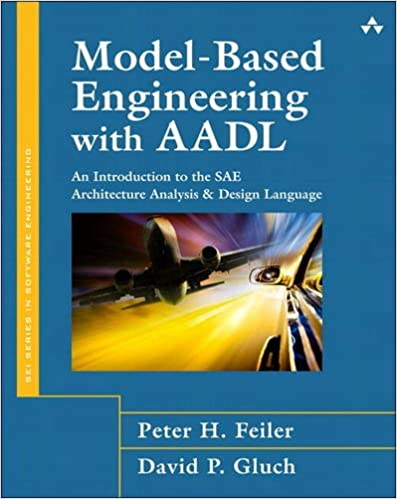
\includegraphics[width=20mm,height=28mm]{book-title-0.jpg}
\hspace*{5mm}

\includegraphics[width=20mm,height=28mm]{book-cover.jpg}


\end{frame}

\begin{frame}\frametitle{AADL in CASE}

AADL is extensible via \emph{annexes}. At Collins we have developed
two annexes used on many projects in the Trusted Systems Group:

\begin{description}
\item [AGREE] SMT-based reasoning over Assume-Guarantee contracts on components
\item [Resolute] Assurance cases as formal entities, using proof search to explore cases.
\end{description}

In CASE, AGREE is used to formulate behavioral security rqts.

Resolute is used for structural properties, and also for linking
results from disparate proof systems.

\end{frame}

\begin{frame}\frametitle{Architecture Transformations}

We have been developing a collection of architecture-to-architecture maps that can be applied to
\emph{provably increase} the security of a system.

\vspace*{4mm}

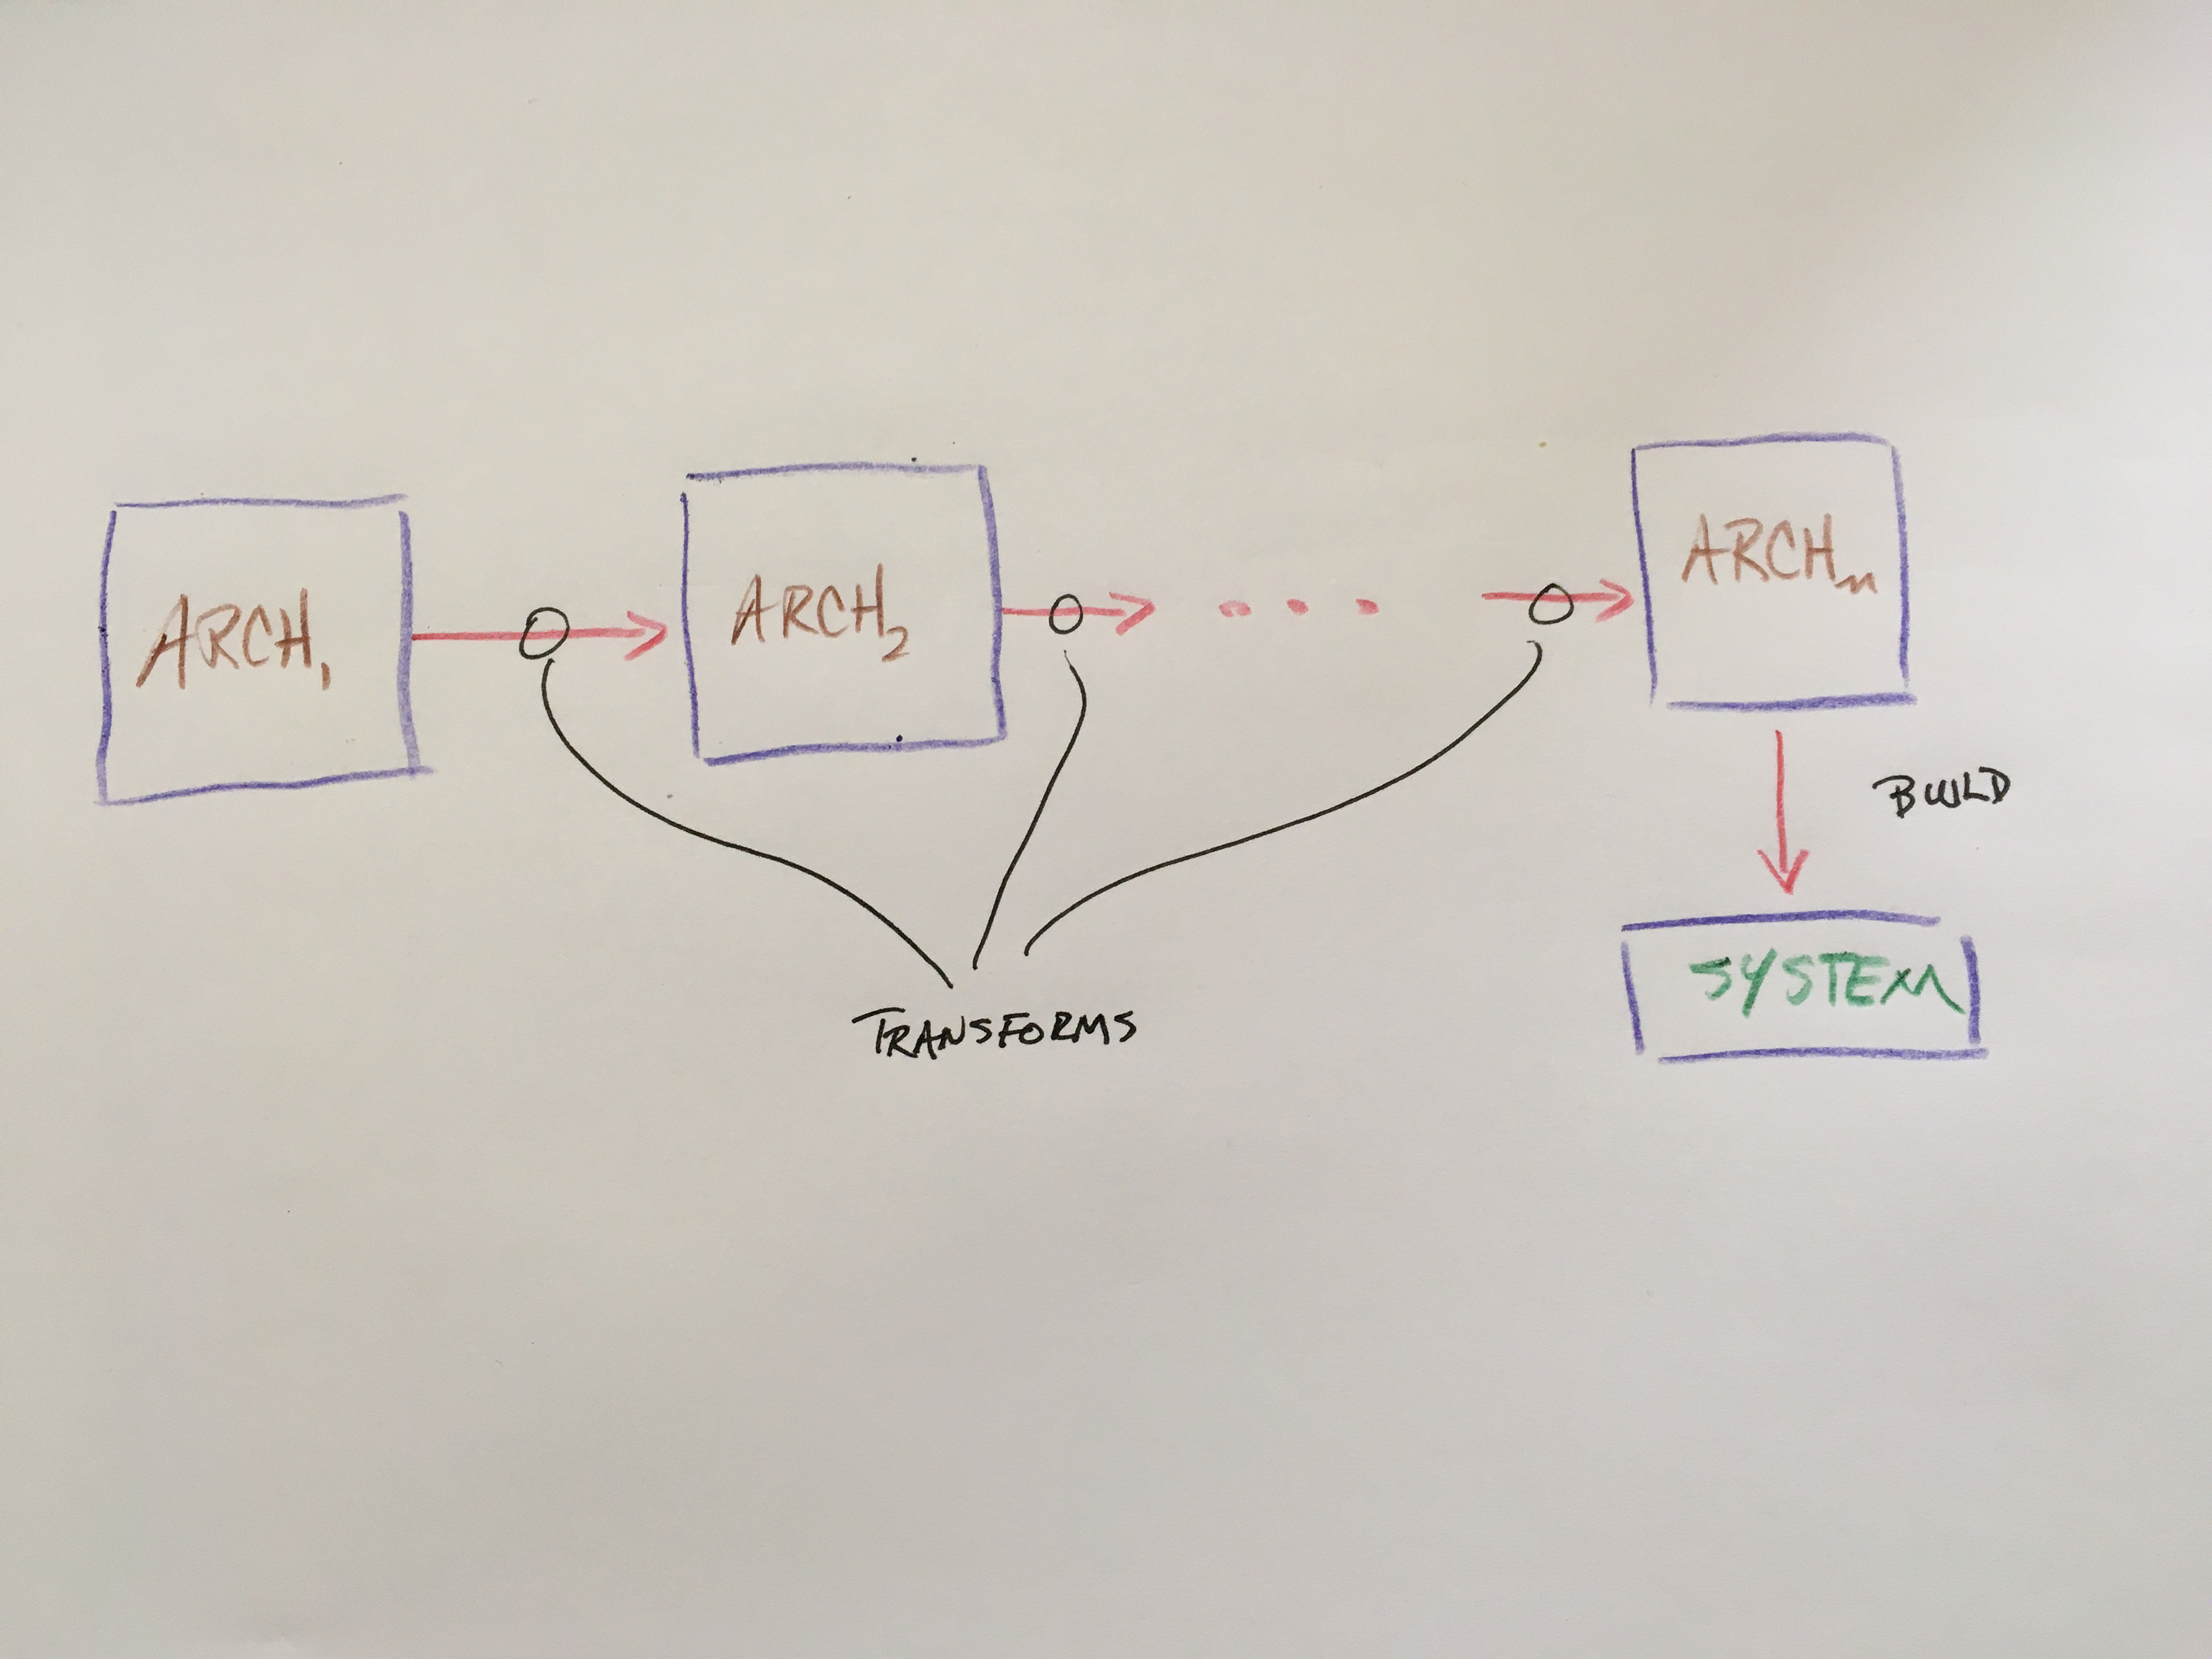
\includegraphics[width=90mm,height=50mm]{arch-trans.jpg}
\end{frame}

\begin{frame}\frametitle{Transformation: Message Filtering}

A \emph{filter} is conceptually very simple: it checks validity of its input data.

\hspace*{10mm}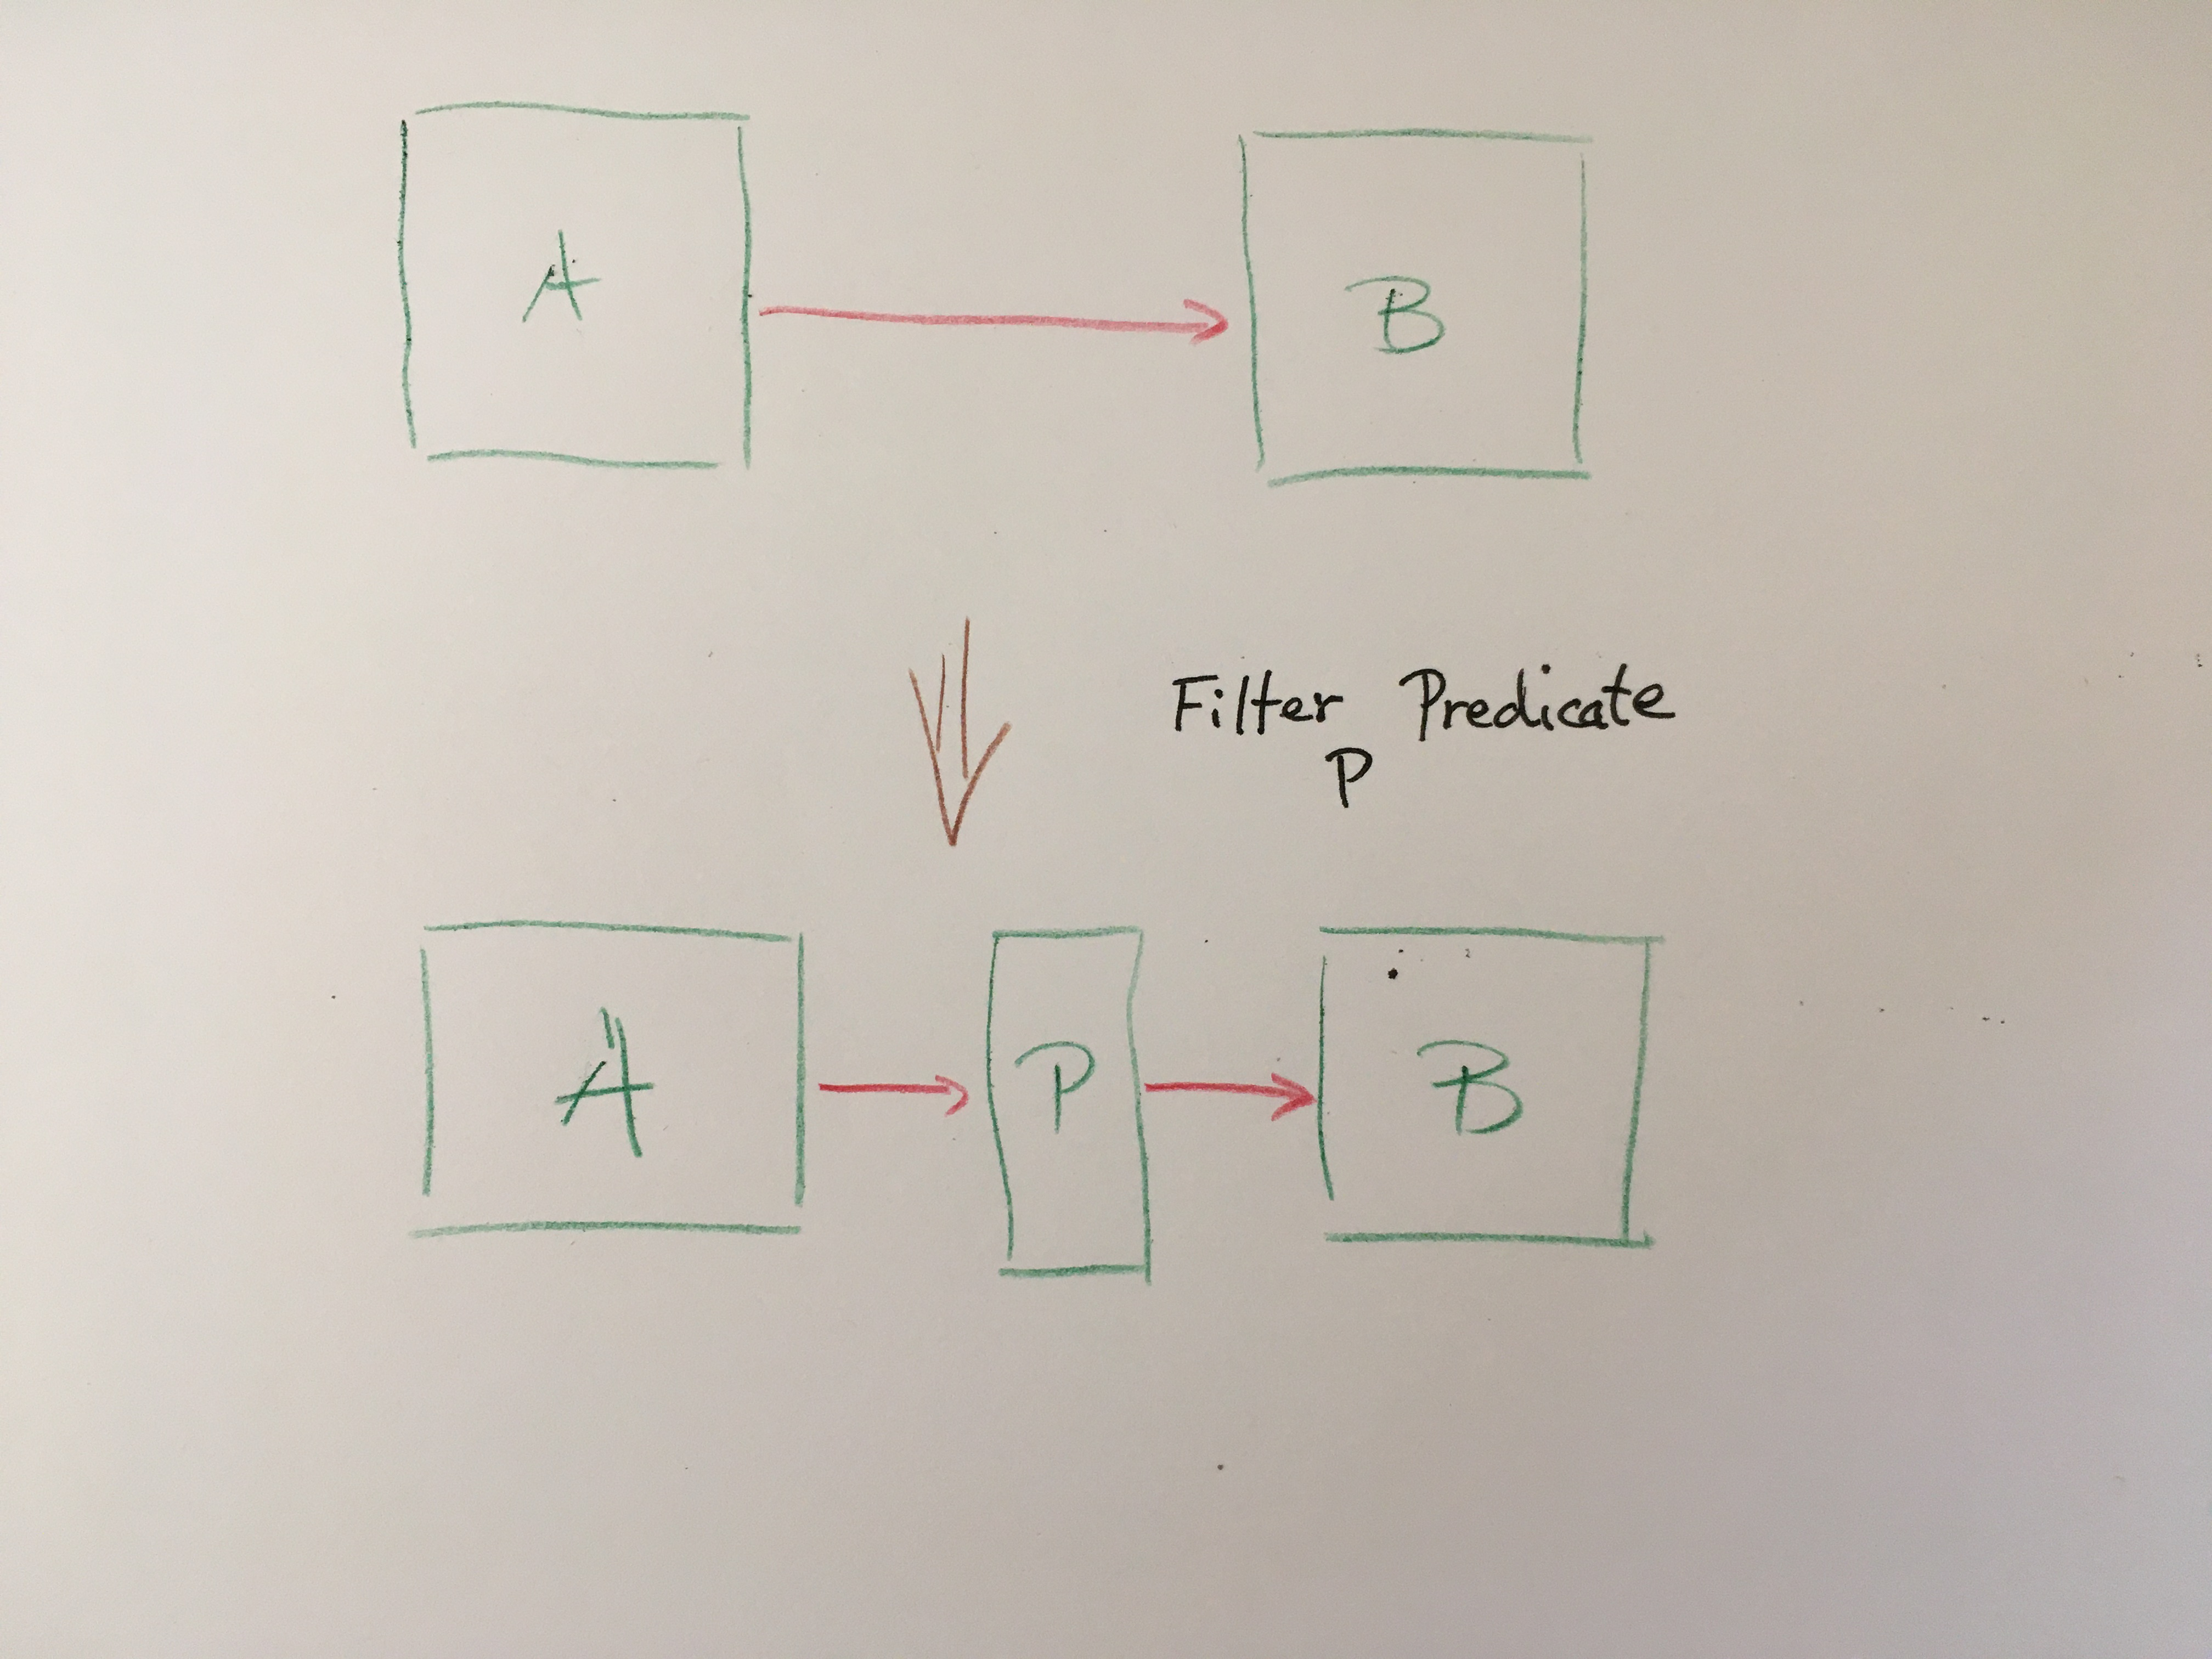
\includegraphics[width=90mm,height=50mm]{filter.jpg}

If the data is valid, then it is passed on. Otherwise it is dropped.

\end{frame}


\begin{frame}\frametitle{Transformation: Message Monitoring}

A \emph{monitor} checks to see that a relationship $\mathcal{R}$ holds
over a collection of message streams through time. If the
specification is violated, an \emph{alert} is sent out.

\hspace*{10mm}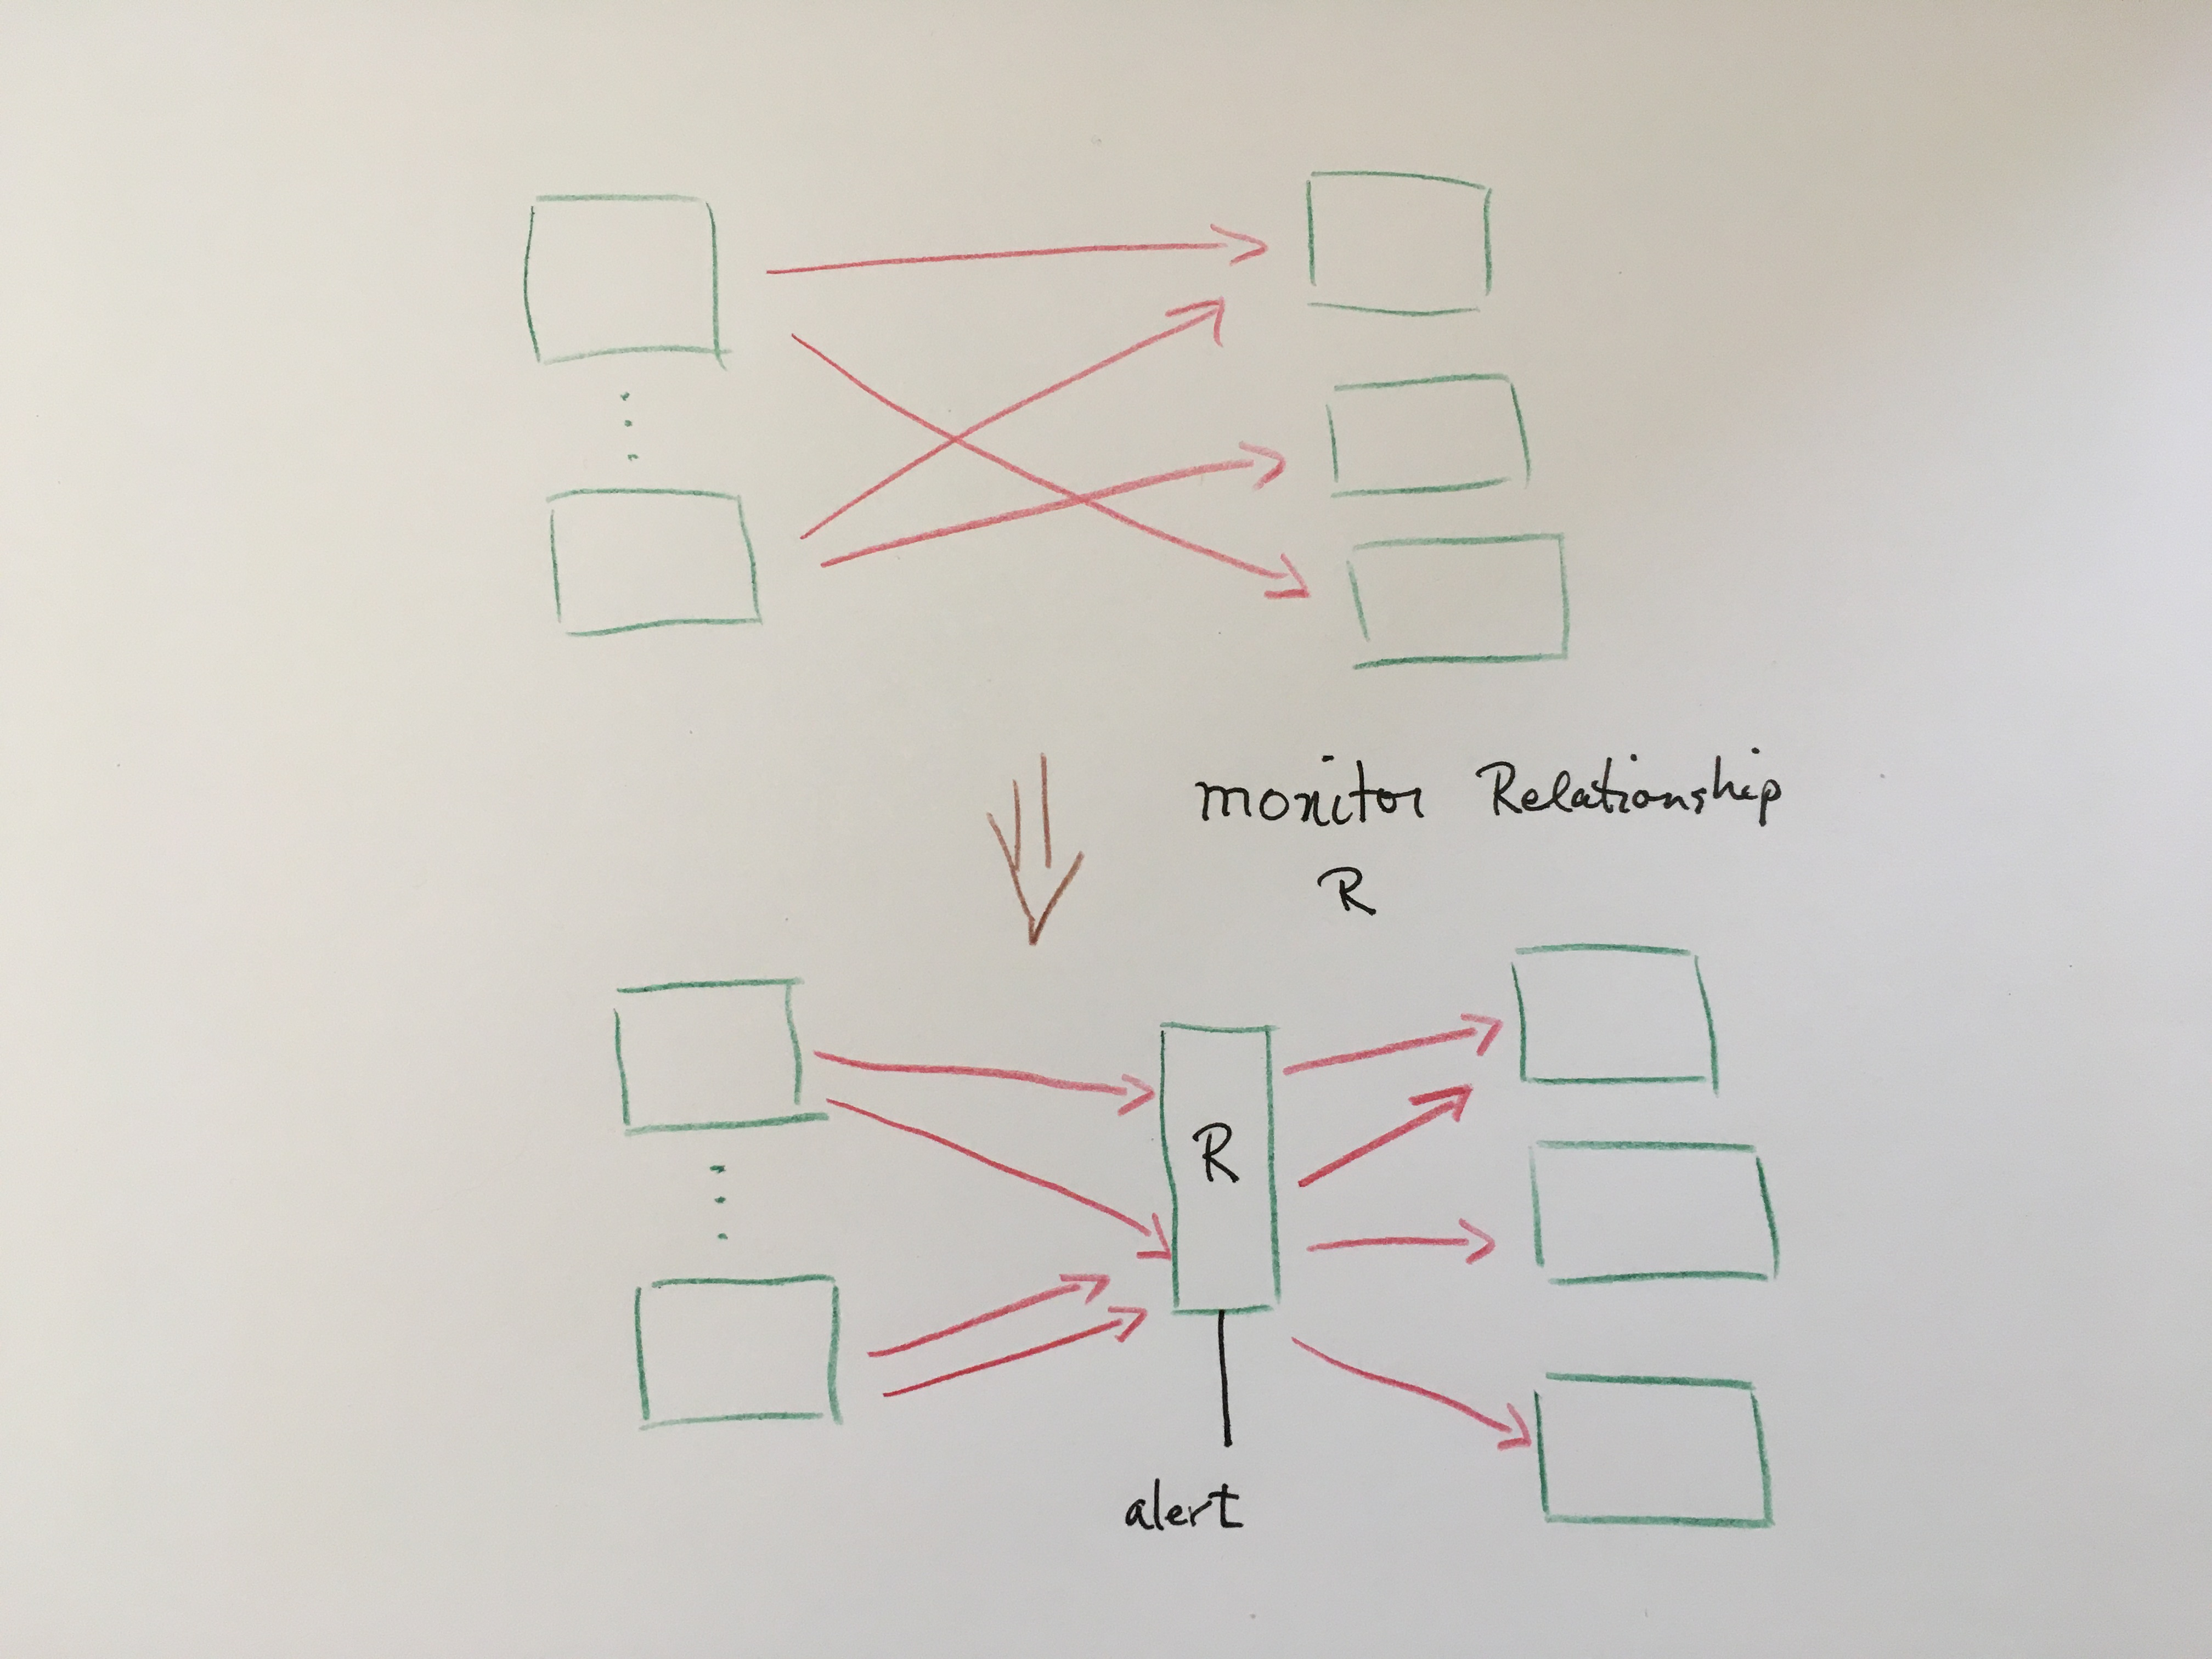
\includegraphics[width=90mm,height=40mm]{monitor.jpg}

We currently use past-time temporal logic to specify monitors

\end{frame}


\begin{frame}\frametitle{Transformation: Isolation of `at risk' components}

An unprotected computational element can be isolated by transparently
lifting it out of its context and mediating access via seL4.

\hspace*{10mm}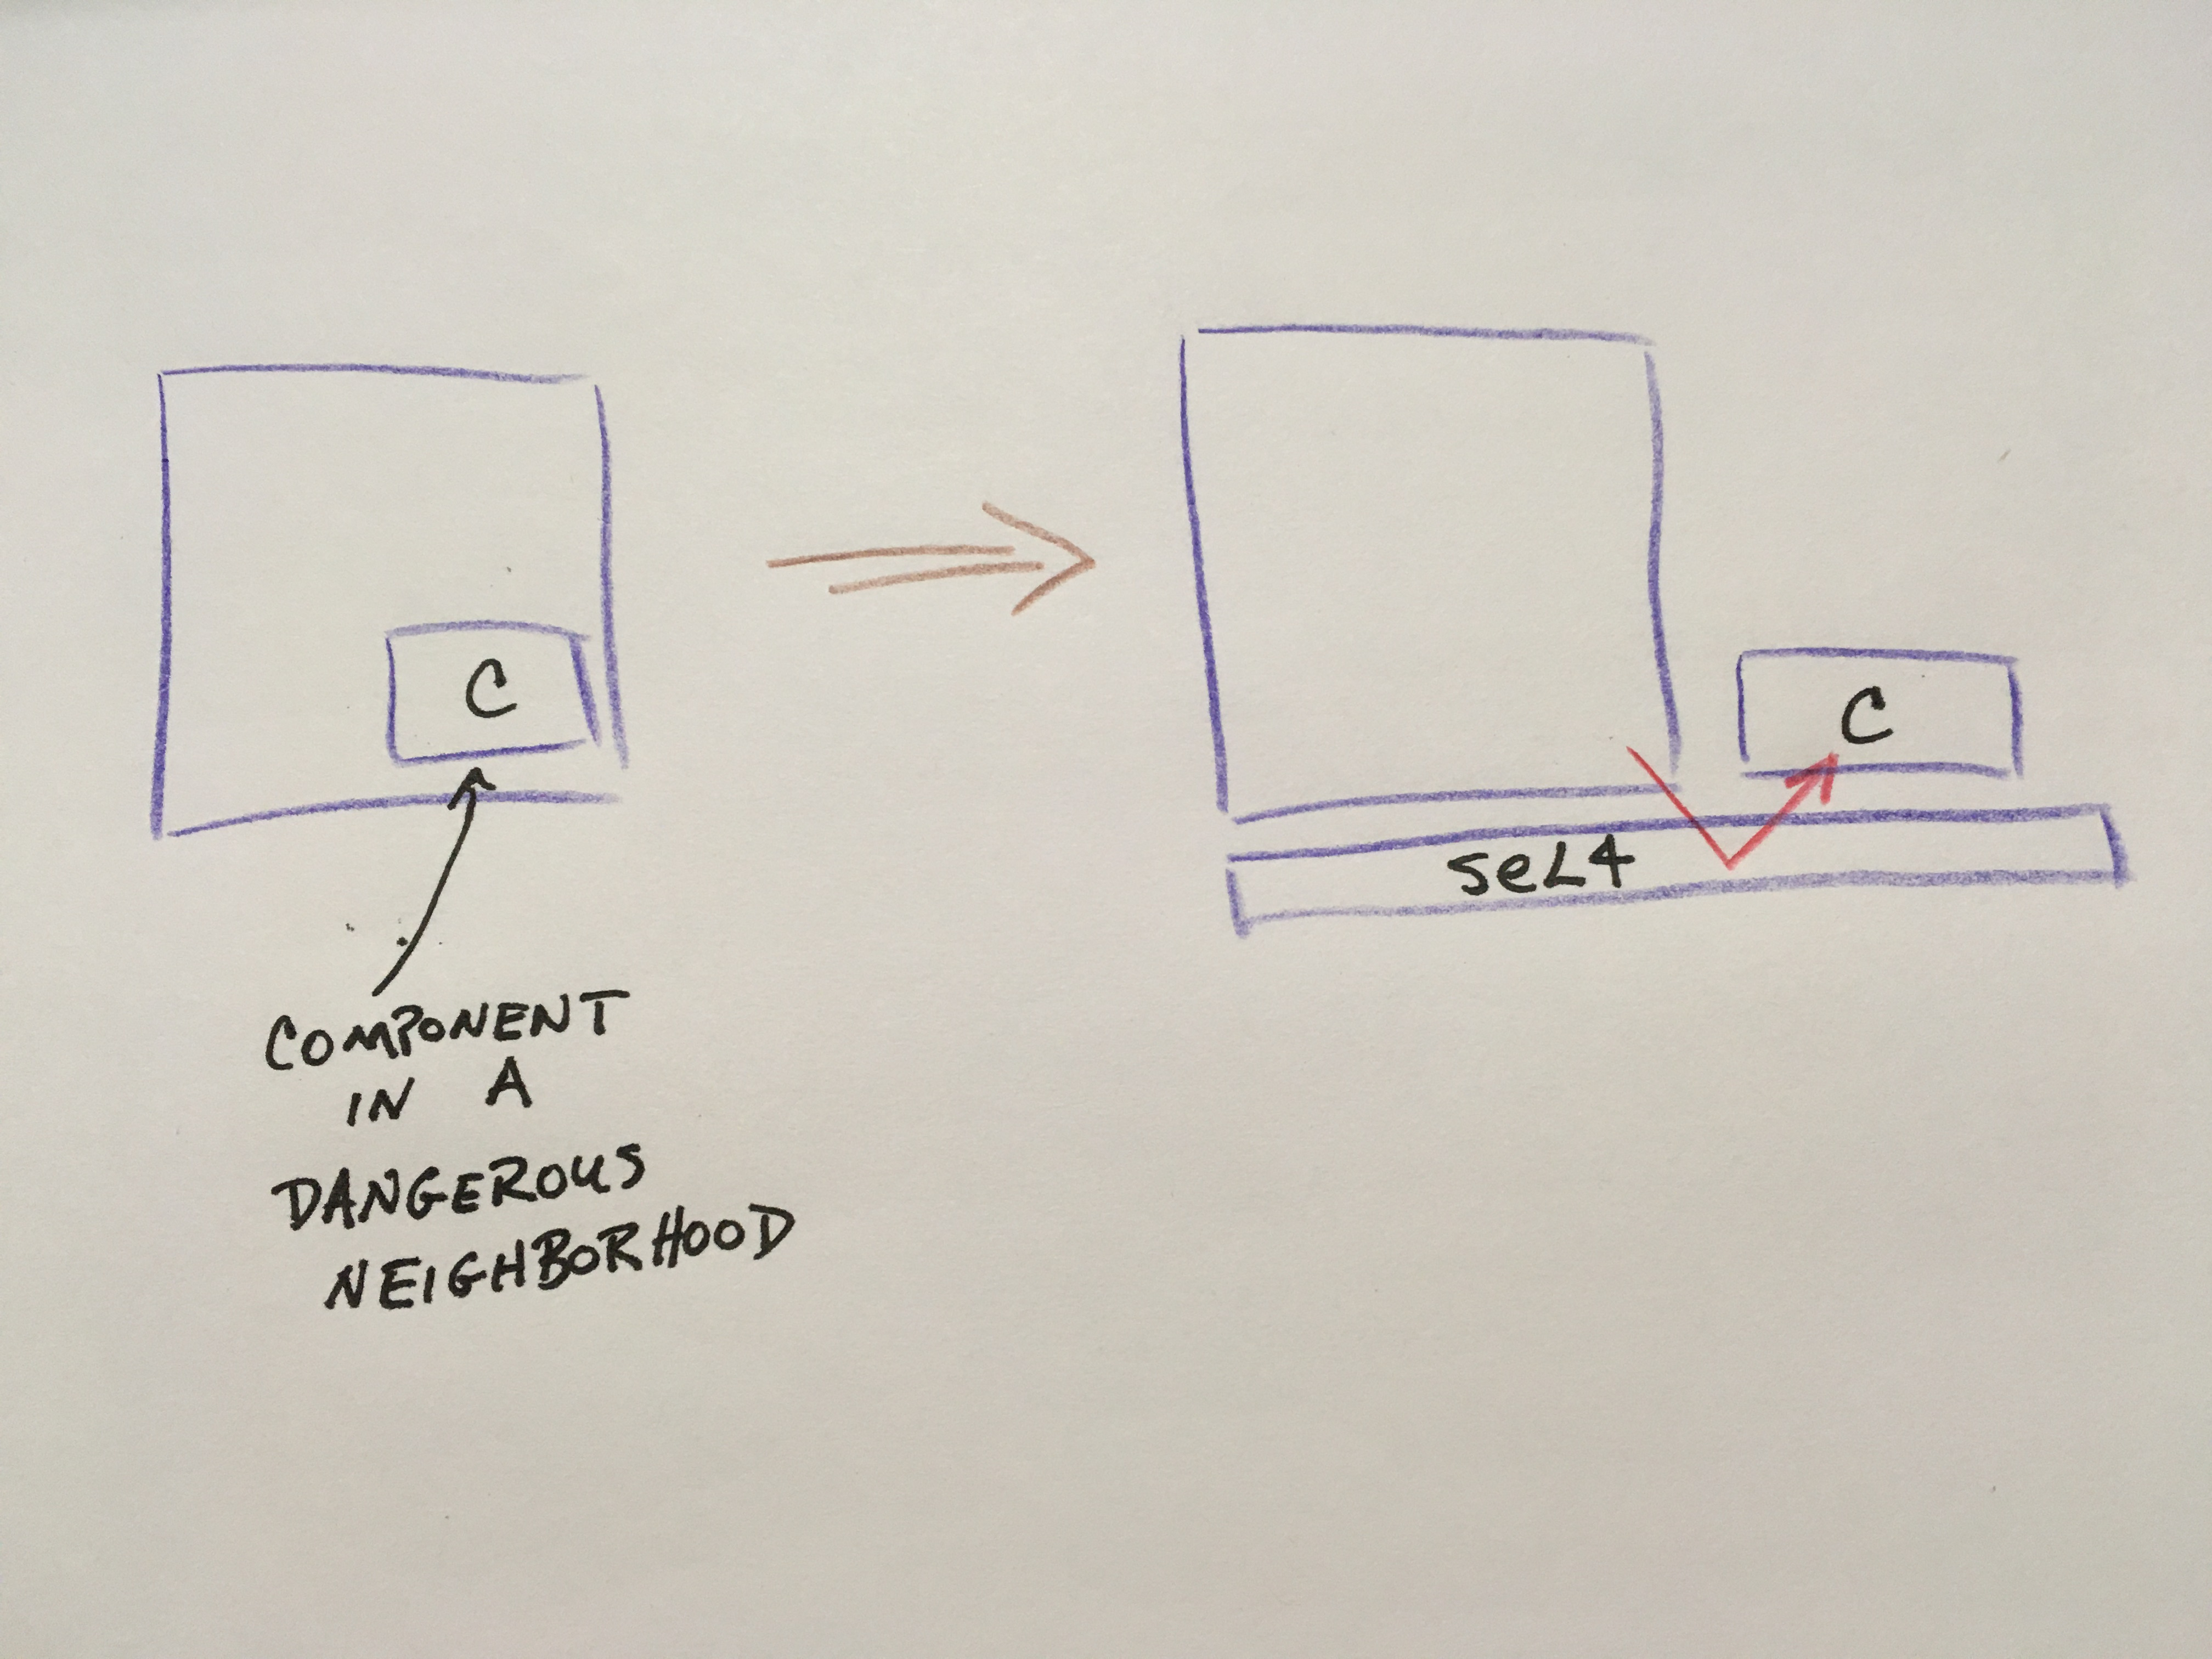
\includegraphics[width=90mm,height=40mm]{vm.jpg}

 Correctness of this transformation depends on formal guarantees provided by seL4.

\end{frame}

\begin{frame}\frametitle{seL4}

\begin{itemize}
\item seL4 microkernel guarantees partitioning of components and
  communication, backed by computer-checked proofs

\item seL4 guarantees no infiltration, exfiltration, eavesdropping,
  interference, and provides fault containment for untrusted code

\end{itemize}

\vspace*{5mm}
\hspace*{10mm}
\includegraphics[width=15mm,height=15mm]{data61-logo.png}
\hspace*{10mm}
\includegraphics[width=15mm,height=15mm]{csiro--black.png}

\end{frame}

\begin{frame}\frametitle{Transformation: Attestation}

Attestation inserts measurement mechanisms into a system. These
examine various aspects of system behavior, and send summaries back to
an observer system.

\hspace*{10mm}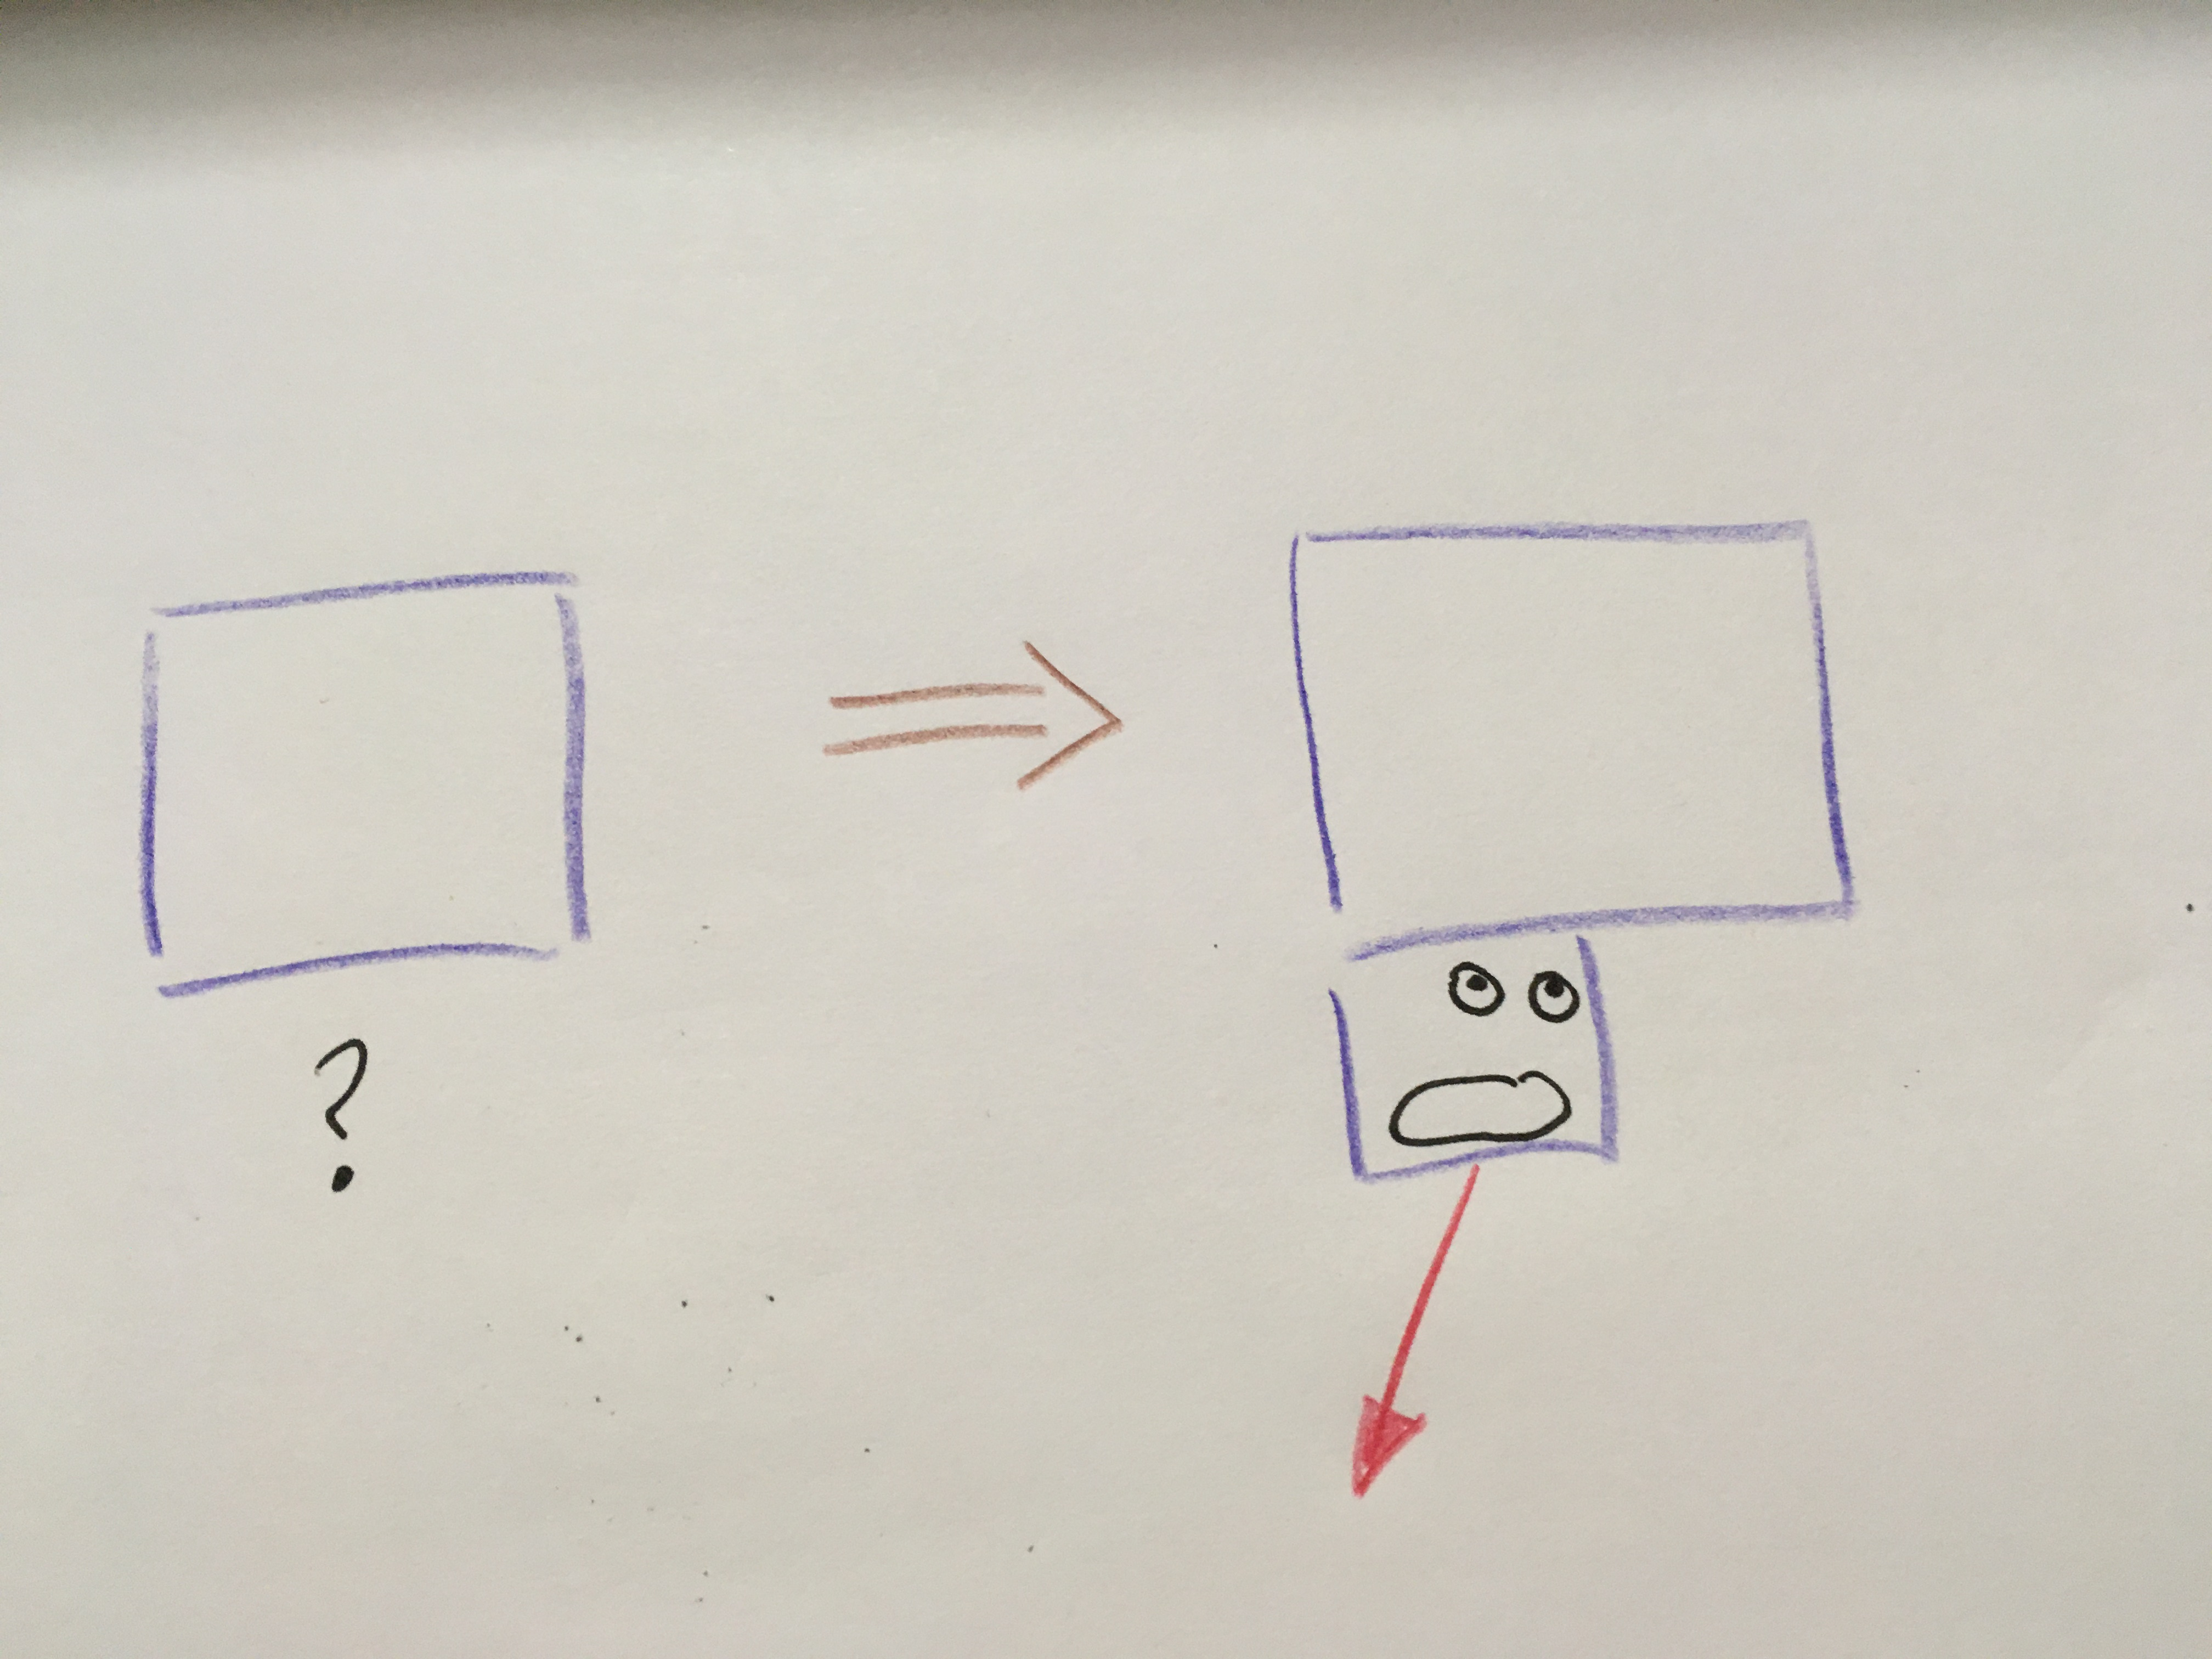
\includegraphics[width=90mm,height=40mm]{att.jpg}

\end{frame}

\begin{frame}[fragile]\frametitle{Example System: uxAS}

 The example we have been using is \textbf{uxAS}, a framework for
 creating autonomous aerial systems from AFRL.

\begin{verbatim}
  https://github.com/afrl-rq/OpenUxAS
\end{verbatim}

\begin{itemize}
\item Open Source
\item Previous experience during the AFRL Summer of Innovation
\item Good setting in which to exercise our ideas
\end{itemize}

\end{frame}

\begin{frame}\frametitle{uxAS system architecture}

The initial system model we start from :

  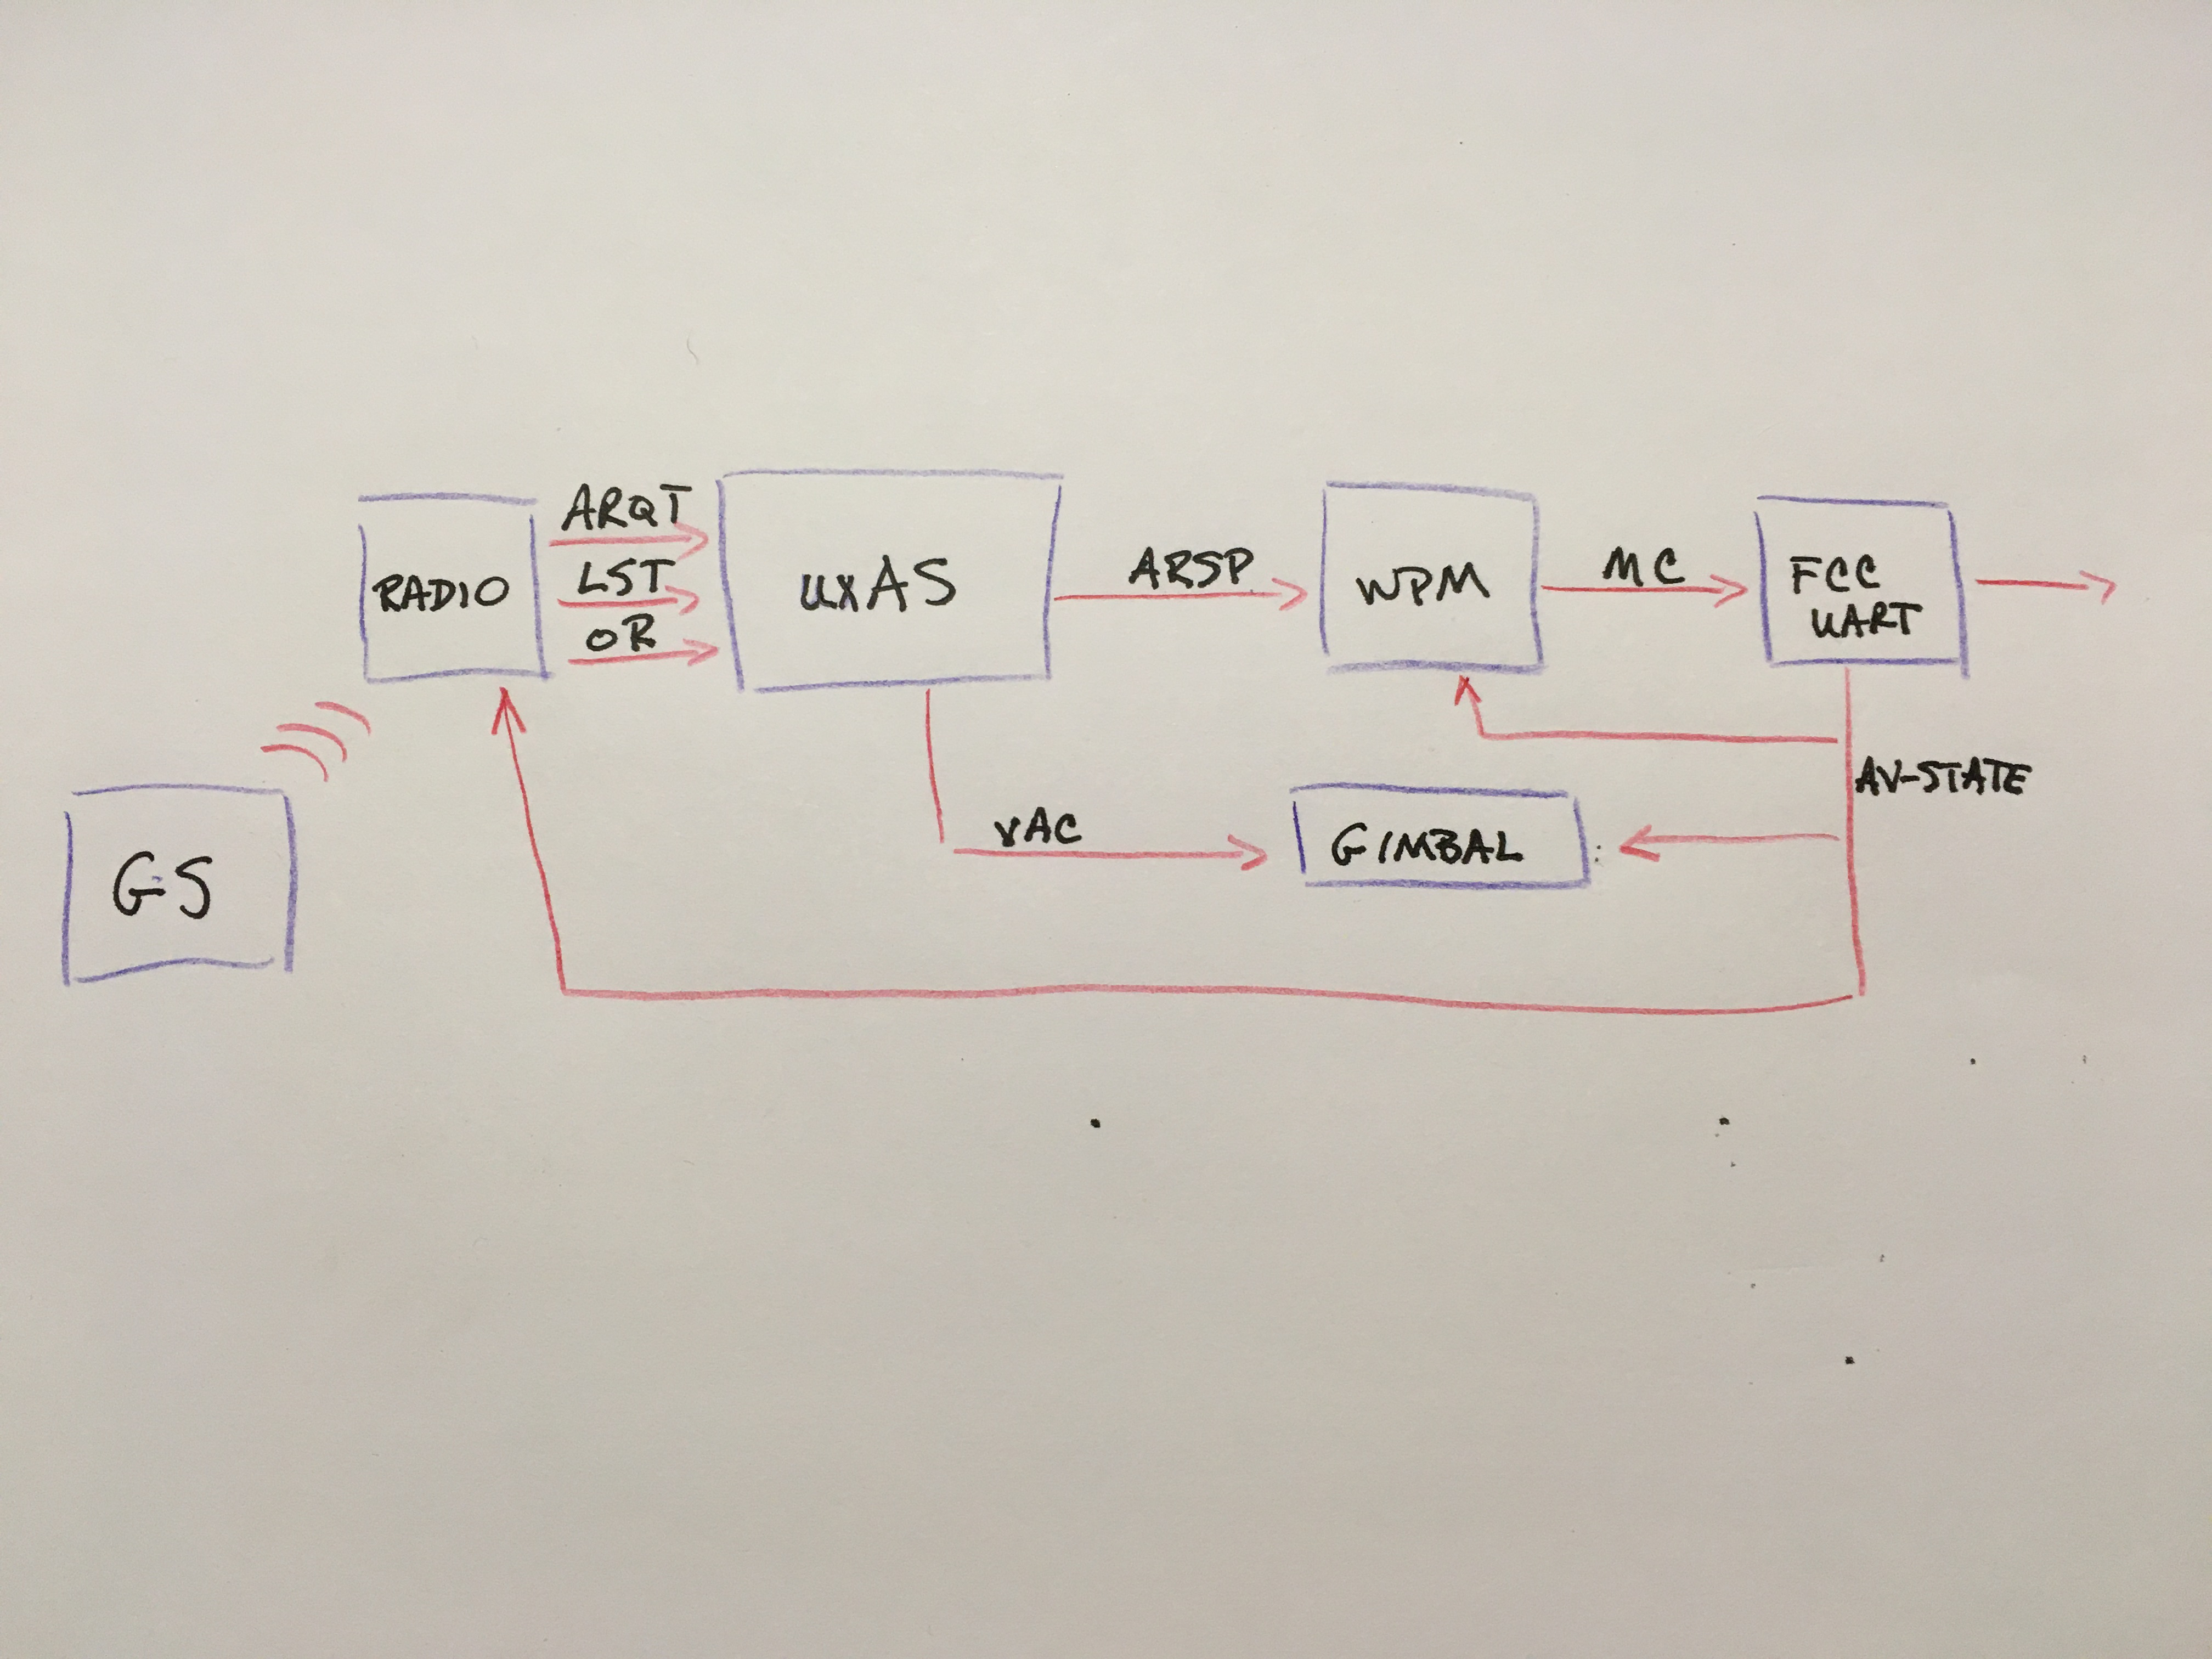
\includegraphics[width=90mm,height=50mm]{uxas-orig.jpg}


\end{frame}

\begin{frame}\frametitle{Notes on the model}

\begin{itemize}
\item UAV is preloaded with a collection of \emph{Operating Regions}
  (Keep-in and Keep-out zones)
\item Commands from GS:
\begin{description}
  \item [OR] Set operating region
  \item [LST] LineSearchTask: \emph{Follow the given sequence of points}
  \item [ARQT] : AutomationRequest: \emph{Create a flight plan to
    achieve a high-level description, e.g., ``surveil the given OR in
    a grid pattern''}
\end{description}

\item Internal messages
\begin{description}
  \item [ARSP]  Response to Automation Request
  \item [VAC]  VehicleActionCommand
  \item [MC]  MissionCommand
  \item [AV-State] AirVehicleState
\end{description}

\end{itemize}

\end{frame}

\begin{frame}\frametitle{Security Considerations}

\begin{itemize}[<+->]
\item \textbf{Problem}: An Operating Region message should designate a known region
\item \textbf{Solution}: Filter OR message to be valid regions

\item \textbf{Problem}: Each point in a Line Search Task should be a valid GPS coordinate
\item \textbf{Solution} Filter LST message on GSP coords

\item \textbf{Problem}: Each point in an Automation Response should be
  in a keep-in zone and not in a keep-out zone
\item \textbf{Solution} Monitor ARSP messages wrt Keep-in and Keep-out zones

\item \textbf{Problem}: Every point in an Automation Response should be a valid GPS coord
\item \textbf{Solution} Filter ARSP message
\end{itemize}

\end{frame}

\begin{frame}\frametitle{Security Considerations continued}

\begin{itemize}[<+->]
\item \textbf{Problem}: Every Automation Request should have a corresponding Response
\item \textbf{Solution}: Monitor ARQT and ARSP for responses matching requests

\item \textbf{Problem}: uxAS software is open source and Waypoint manager could be compromised
\item \textbf{Solution}: Isolate Waypoint Manager on a VM

\item \textbf{Problem}: Ground station could be compromised; UAV needs to defend itself against that
\item \textbf{Solution}: Attestation Manager on GS, talking to UAV
\end{itemize}

\end{frame}


\begin{frame}\frametitle{Transformed uxAS}

The transformed model :

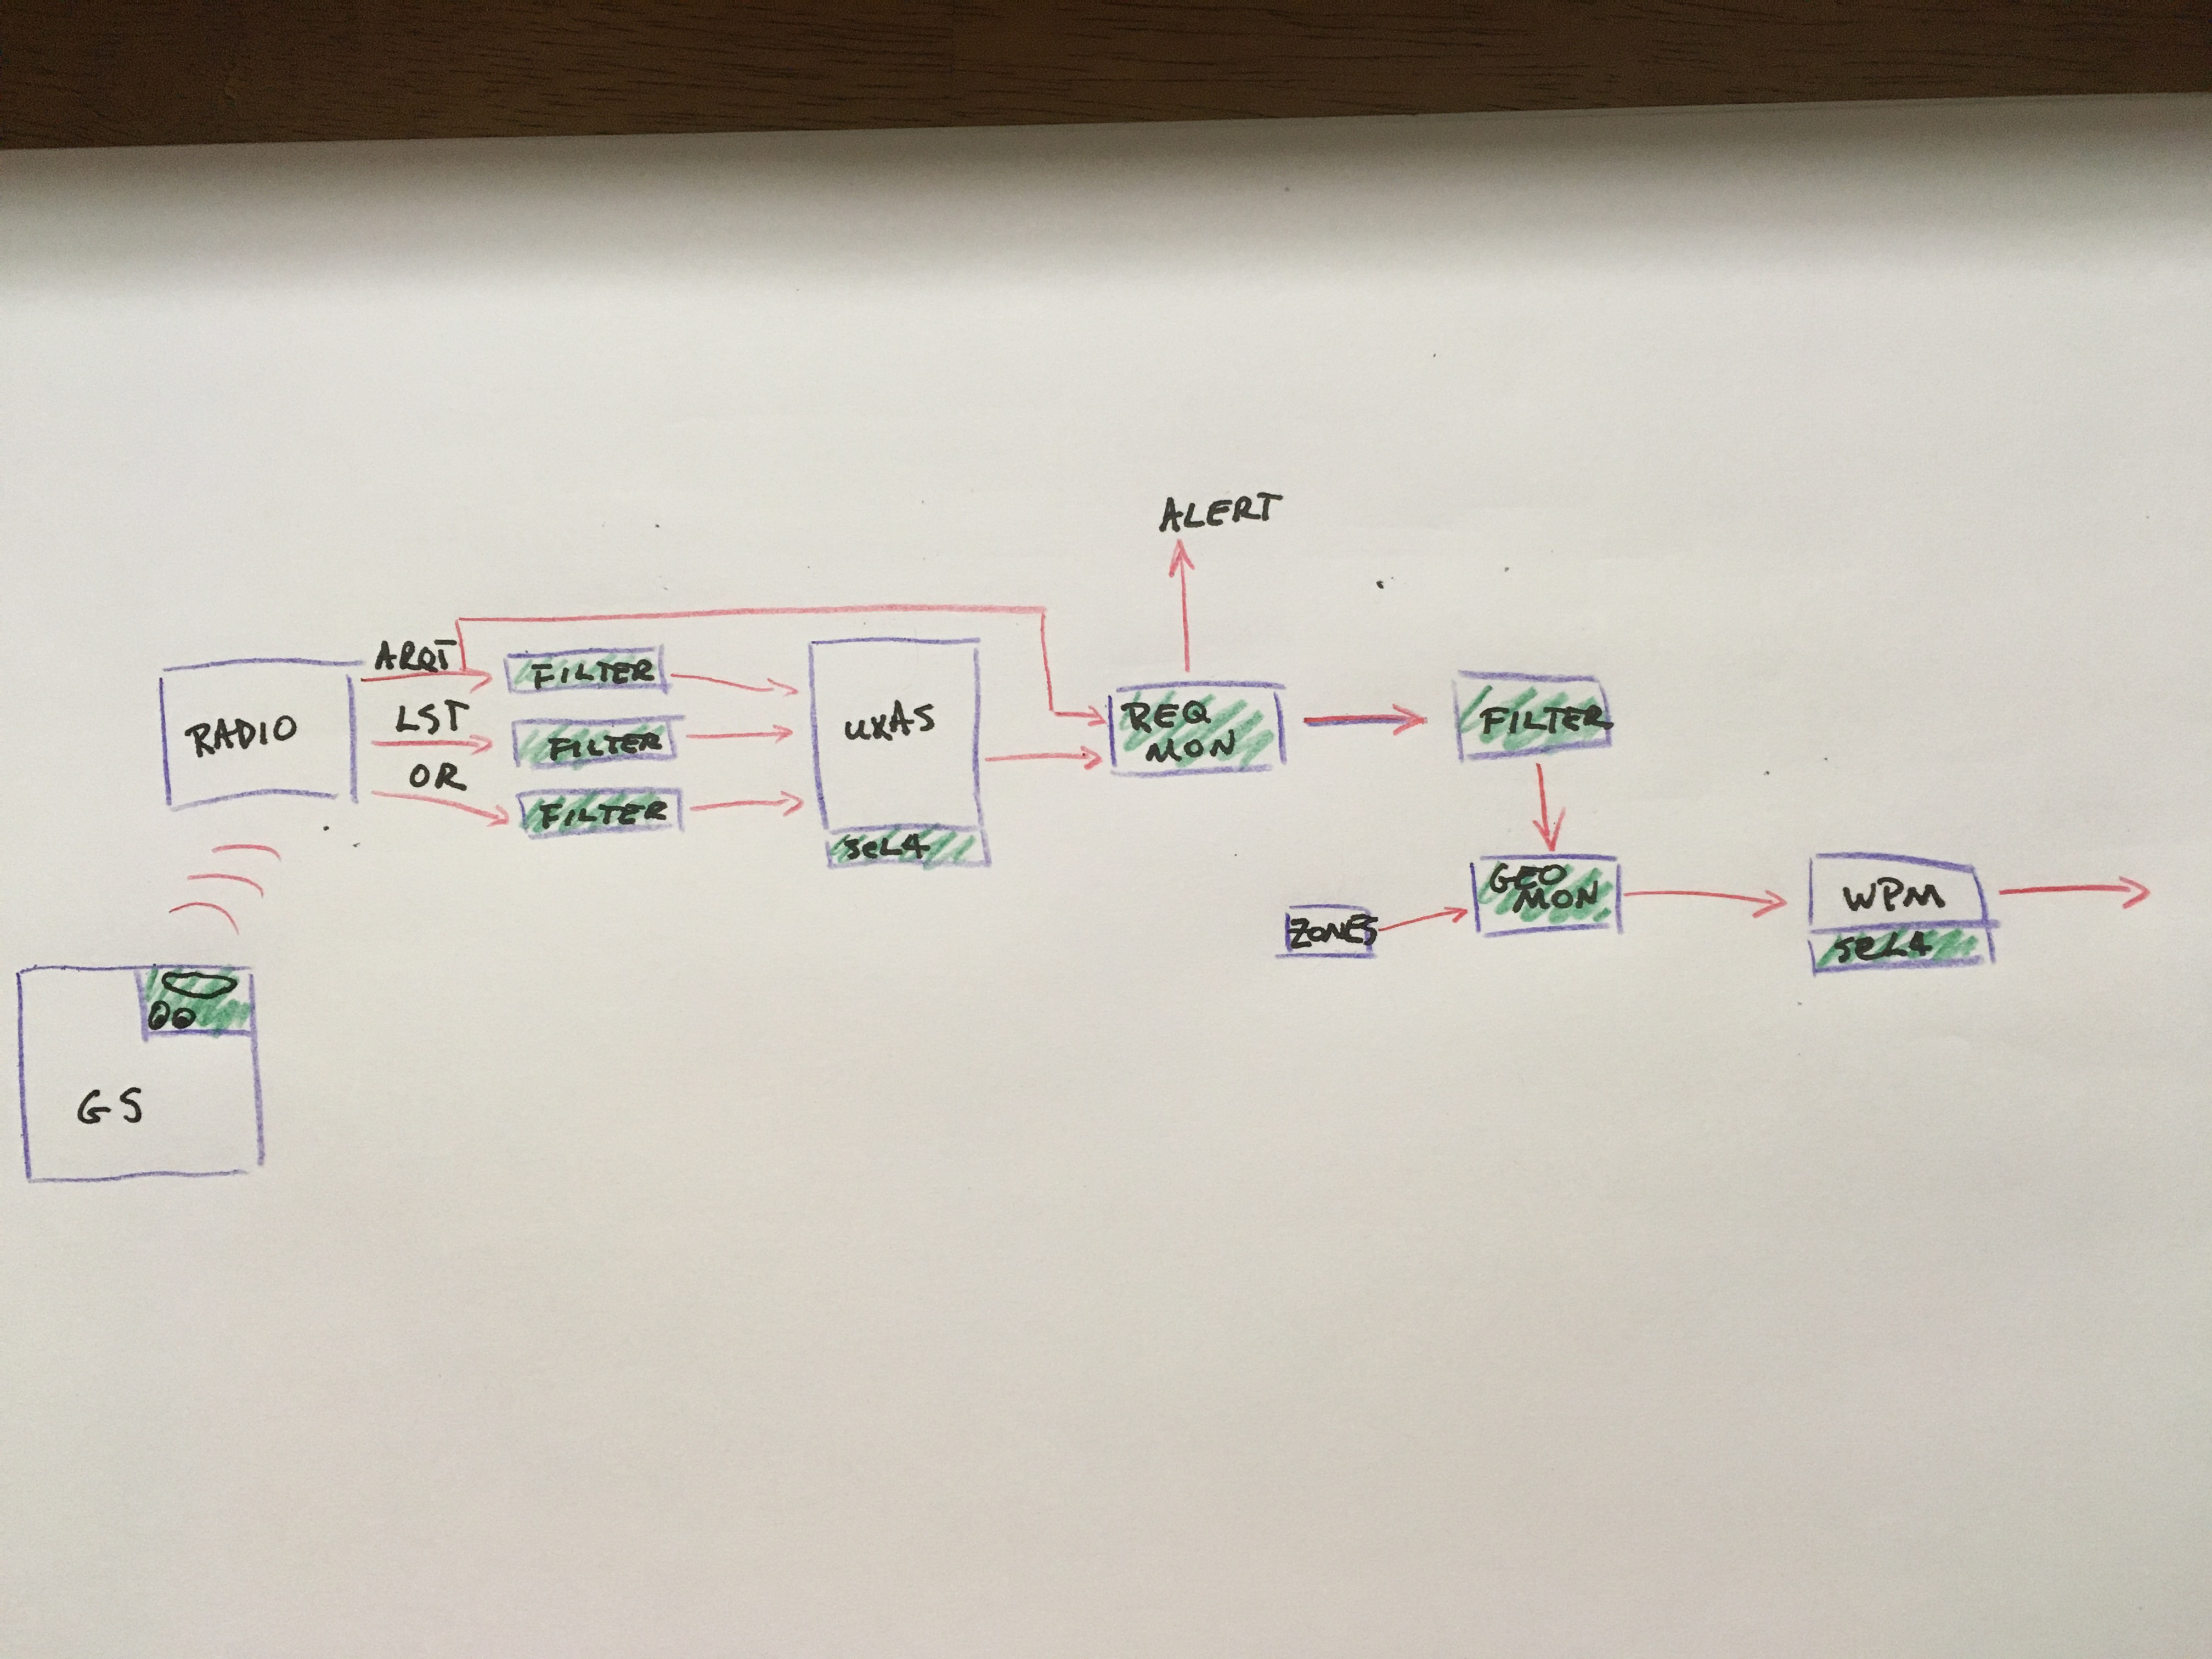
\includegraphics[width=90mm,height=50mm]{final-arch.jpg}

\end{frame}

\begin{frame}\frametitle{Implementations and Build}

As the transformations are applied, implementations and
configuration information are generated.

\begin{itemize}

  \item For ``simple'' transformations code can be generated at transformation time.
  \item For the VM and Attestation transforms, configuration
    information can be generated, but the details of the
    implementation are more involved.
\end{itemize}

Finally the \textbf{BUILD} can now be invoked.


\includegraphics[width=20mm,height=20mm]{ksu.jpg}

\includegraphics[width=20mm,height=20mm]{adventium.png}


\end{frame}

\begin{frame}\frametitle{Build}

The build is very challenging. The \textbf{HAMR} toolsuite implements
multi-stage translation architecture to address the following goals:
\begin{itemize}

\item Semantic consistency from model to execution ensures model-level
  analysis applies to deployed code

\item Build for multiple target platforms: seL4, Linux

\item Same computational model across different platforms

\item Same semantics for threading and communication

\end{itemize}

\end{frame}

\begin{frame}\frametitle{Summary}

System designer uses OSATE, using menus to specify and configure transforms.

The interface makes sanity checks and sets up for the eventual system build

Once implementations are created for the new system components, we
have to guard against increasing the attack surface of the system.

Formal specification and proof to the rescue! (Mostly.)

\end{frame}

\section {Deep Dive: Message Filters}

\begin{frame}\frametitle{Ports and Messages}

Question: what does a filter operate over?

\begin{itemize}

  \item An AADL component communicates with other components via \emph{connections}

\item  An endpoint (port) on a connection has a \emph{type} (booleans,
  integers, floats, arrays, unions, ...)

\item Properties in AGREE (our specification language) are therefore written over these types.

\item However, in the implementation, messages coming into a port are
  byte arrays (essentially untyped)

\end{itemize}

\end{frame}

\begin{frame}[fragile]\frametitle{Example : Wellformed GPS coordinates in AGREE}

{\small
\begin{verbatim}
 AltitudeType = AGL | MSL

 Location3D = {
  Latitude  : real64,
  Longitude : real64,
  Altitude  : real32,
  AltitudeType : AltitudeType}

 Good_Location (loc) =
    -90.0 <= loc.Latitude <= 90.0 and
   -180.0 <= loc.Longitude <= 180.0 and
      0.0 <= loc.Altitude <= 15000.0
\end{verbatim}
}

\end{frame}

\begin{frame}\frametitle{Example : Wellformed GPS strings}

\[
\begin{array}{l}
 \konst{Good\_Location\_String} (s) \iff \\
\quad   \exists s_1 s_2 s_3 s_4. \\
\qquad      s = s1 \bullet s2 \bullet s3 \bullet s4 \ \land \\
\qquad    -90.0 \leq \konst{doubleVal}(s1) \leq 90.0 \ \land \\
\qquad   -180.0 \leq \konst{doubleVal}(s2) \leq 180.0 \ \land \\
\qquad      0.0 \leq \konst{floatVal}(s3)  \leq 15000.0 \ \land \\
\qquad        0 \leq \konst{natVal}(s4) \leq 1
\end{array}
\]

\noindent where

\[
\begin{array}{ll}
 \konst{doubleVal} & : \konst{string} \to \konst{double} \\
 \konst{floatVal}  & : \konst{string} \to \konst{float}  \\
 \konst{natVal}    & : \konst{string} \to \konst{nat}  \\
\end{array}
\]

\end{frame}

\begin{frame}\frametitle{SPLAT}

We need to span the gap between high level data and flat strings.

Our approach : \textbf{SPLAT} (Semantic Properties for Language and Automata Theory)

Try to apply ideas from Formal Language Theory to showing properties
of operations on high-level data.

\end{frame}


\begin{frame}[fragile]\frametitle{Contiguity Types}

The goal is to automatically generate an implementation of the
well-formedness predicate \verb+Good_Location+ from its specification.

There is a problem : the encoding from datastructures to strings is not specified.

For uxAs, this is a fairly complex encoding.

We specify the message format using \emph{contiguity types}. With this representation we can
\begin{itemize}
\item automatically generate message filters and parsers
\item automatically prove that the filter has the desired property (\verb+Good_Location_String+ in our example)
\end{itemize}

\end{frame}

\begin{frame}[fragile]\frametitle{uxAS LineSearchTask messages}

  Message formats can be arbitrarily complex, and usually include
  features such as variable-length arrays, and unions.

  {\small
\begin{verbatim}
  {TaskID :           i64,
   Label :            uxasString,
   EligibleEntities : uxasBoundedArray i64 32,
   RevisitRate :      real32,
   Parameters :       uxasBoundedArray (mesgOption "KEYVALUEPAIR" keyValuePair) 8,
   Priority :         u8,
   Required :         bool,
   DesiredWavelengthBands : uxasBoundedArray uxasWavelengthBand 8,
   DwellTime :              i64,
   GroundSampleDistance :   real32,
   PointList :     uxasBoundedArray (mesgOption "LOCATION3D" location3D) 1024,
   ViewAngleList : uxasBoundedArray (mesgOption "WEDGE" wedge) 16,
   UseInertialViewAngles : bool
\end{verbatim}
}
\end{frame}

\begin{frame}[fragile]\frametitle{Contiguity Types: Syntax}

The syntax of contiguity types is very similar to a standard
collection of base types closed under formation of records and arrays.

\[
\begin{array}{rcl}
 \mathit{base} & = & \konst{bool} \mid \konst{char} \mid \konst{u8} \mid
 \konst{u16} \mid \konst{u32} \mid \konst{u64}  \mid \konst{i16} \mid
 \konst{i32} \mid \konst{i64} \mid \konst{f32} \mid \konst{f64} \\
 \tau & = & \mathit{base} \\
      & \mid & \konst{Recd}\; (f_1 : \tau_1) \ldots (f_n : \tau_n) \\
      & \mid & \konst{Array}\; \tau \; \mathit{exp} \\
      & \mid & \konst{Union}\; (\mathit{bexp}_1 : \tau_1) \ldots (\mathit{bexp}_n : \tau_n)
\end{array}
\]
\end{frame}


\begin{frame}[fragile]\frametitle{Contiguity Types: Semantics}

The semantics of contiguity types is in terms of formal languages
(sets of strings):

\[
% \begin{array}{l}
\LangTheta{\tau} =
\mathtt{case}\; \tau\
% \hspace*{3mm}
 \left\{
 \begin{array}{l}
 \mathit{base} \Rightarrow \set{s \mid \konst{len}(s) = \konst{width}(base)} \\
 \konst{Recd}\; (f_1 : \tau_1) \ldots (f_n : \tau_n)
      \Rightarrow \LangTheta{\tau_1} \cdot \ldots \cdot \LangTheta{\tau_n}
\\
 \konst{Array}\; \tau_1 \; \mathit{exp}
      \Rightarrow  \LangTheta{\tau_1}^{\konst{evalExp}\;\theta\;\mathit{exp}}
\\
 \konst{Union}\; (\mathit{bexp}_1 : \tau_1) \ldots (\mathit{bexp}_n : \tau_n) \Rightarrow \\
  \hspace*{5mm}
 \left\{
 \begin{array}{ll}
    \LangTheta{\tau_i} &  \mathrm{if}\ \konst{evalBexp}\;\theta\;\mathit{bexp}_i = \konst{true} \\
                  & \mathrm{and\ no\ other}\ \mathit{bexp}_j\ \mathrm{is}\ \konst{true}  \\
    \emptyset & \mathrm{otherwise}
 \end{array}
 \right.
 \\
\end{array}
 \right.
%\end{array}
\]
\end{frame}

\begin{frame}[fragile]\frametitle{Correctness of parameterized matcher}

We can define a function \textbf{match} which takes a contig type and
a string and returns an assignment of slices of the string to elements of the type.

\begin{theorem}[Correctness]
  \[
 \vdash \konst{match}\; \mathit{contig}\; \mathit{string} = \konst{Some}(\theta) \imp
   \mathit{string} \in \LangTheta{\mathit{contig}}
\]
\end{theorem}

\textbf{match} has the flavor of a \emph{parser generator}: it takes a
specification of the language to be parsed and returns an implementation

We use \textbf{match} to implement all filters in the transformed uxAS
and parsers for the monitors.

\end{frame}

\section {Assembling a Security Case}

\begin{frame}\frametitle{Joining theorems together}

  We can join the correctness of the message matcher with the
  correctness of the CakeML toolchain to obtain a \emph{single-shot} correctness theorem in HOL4:

  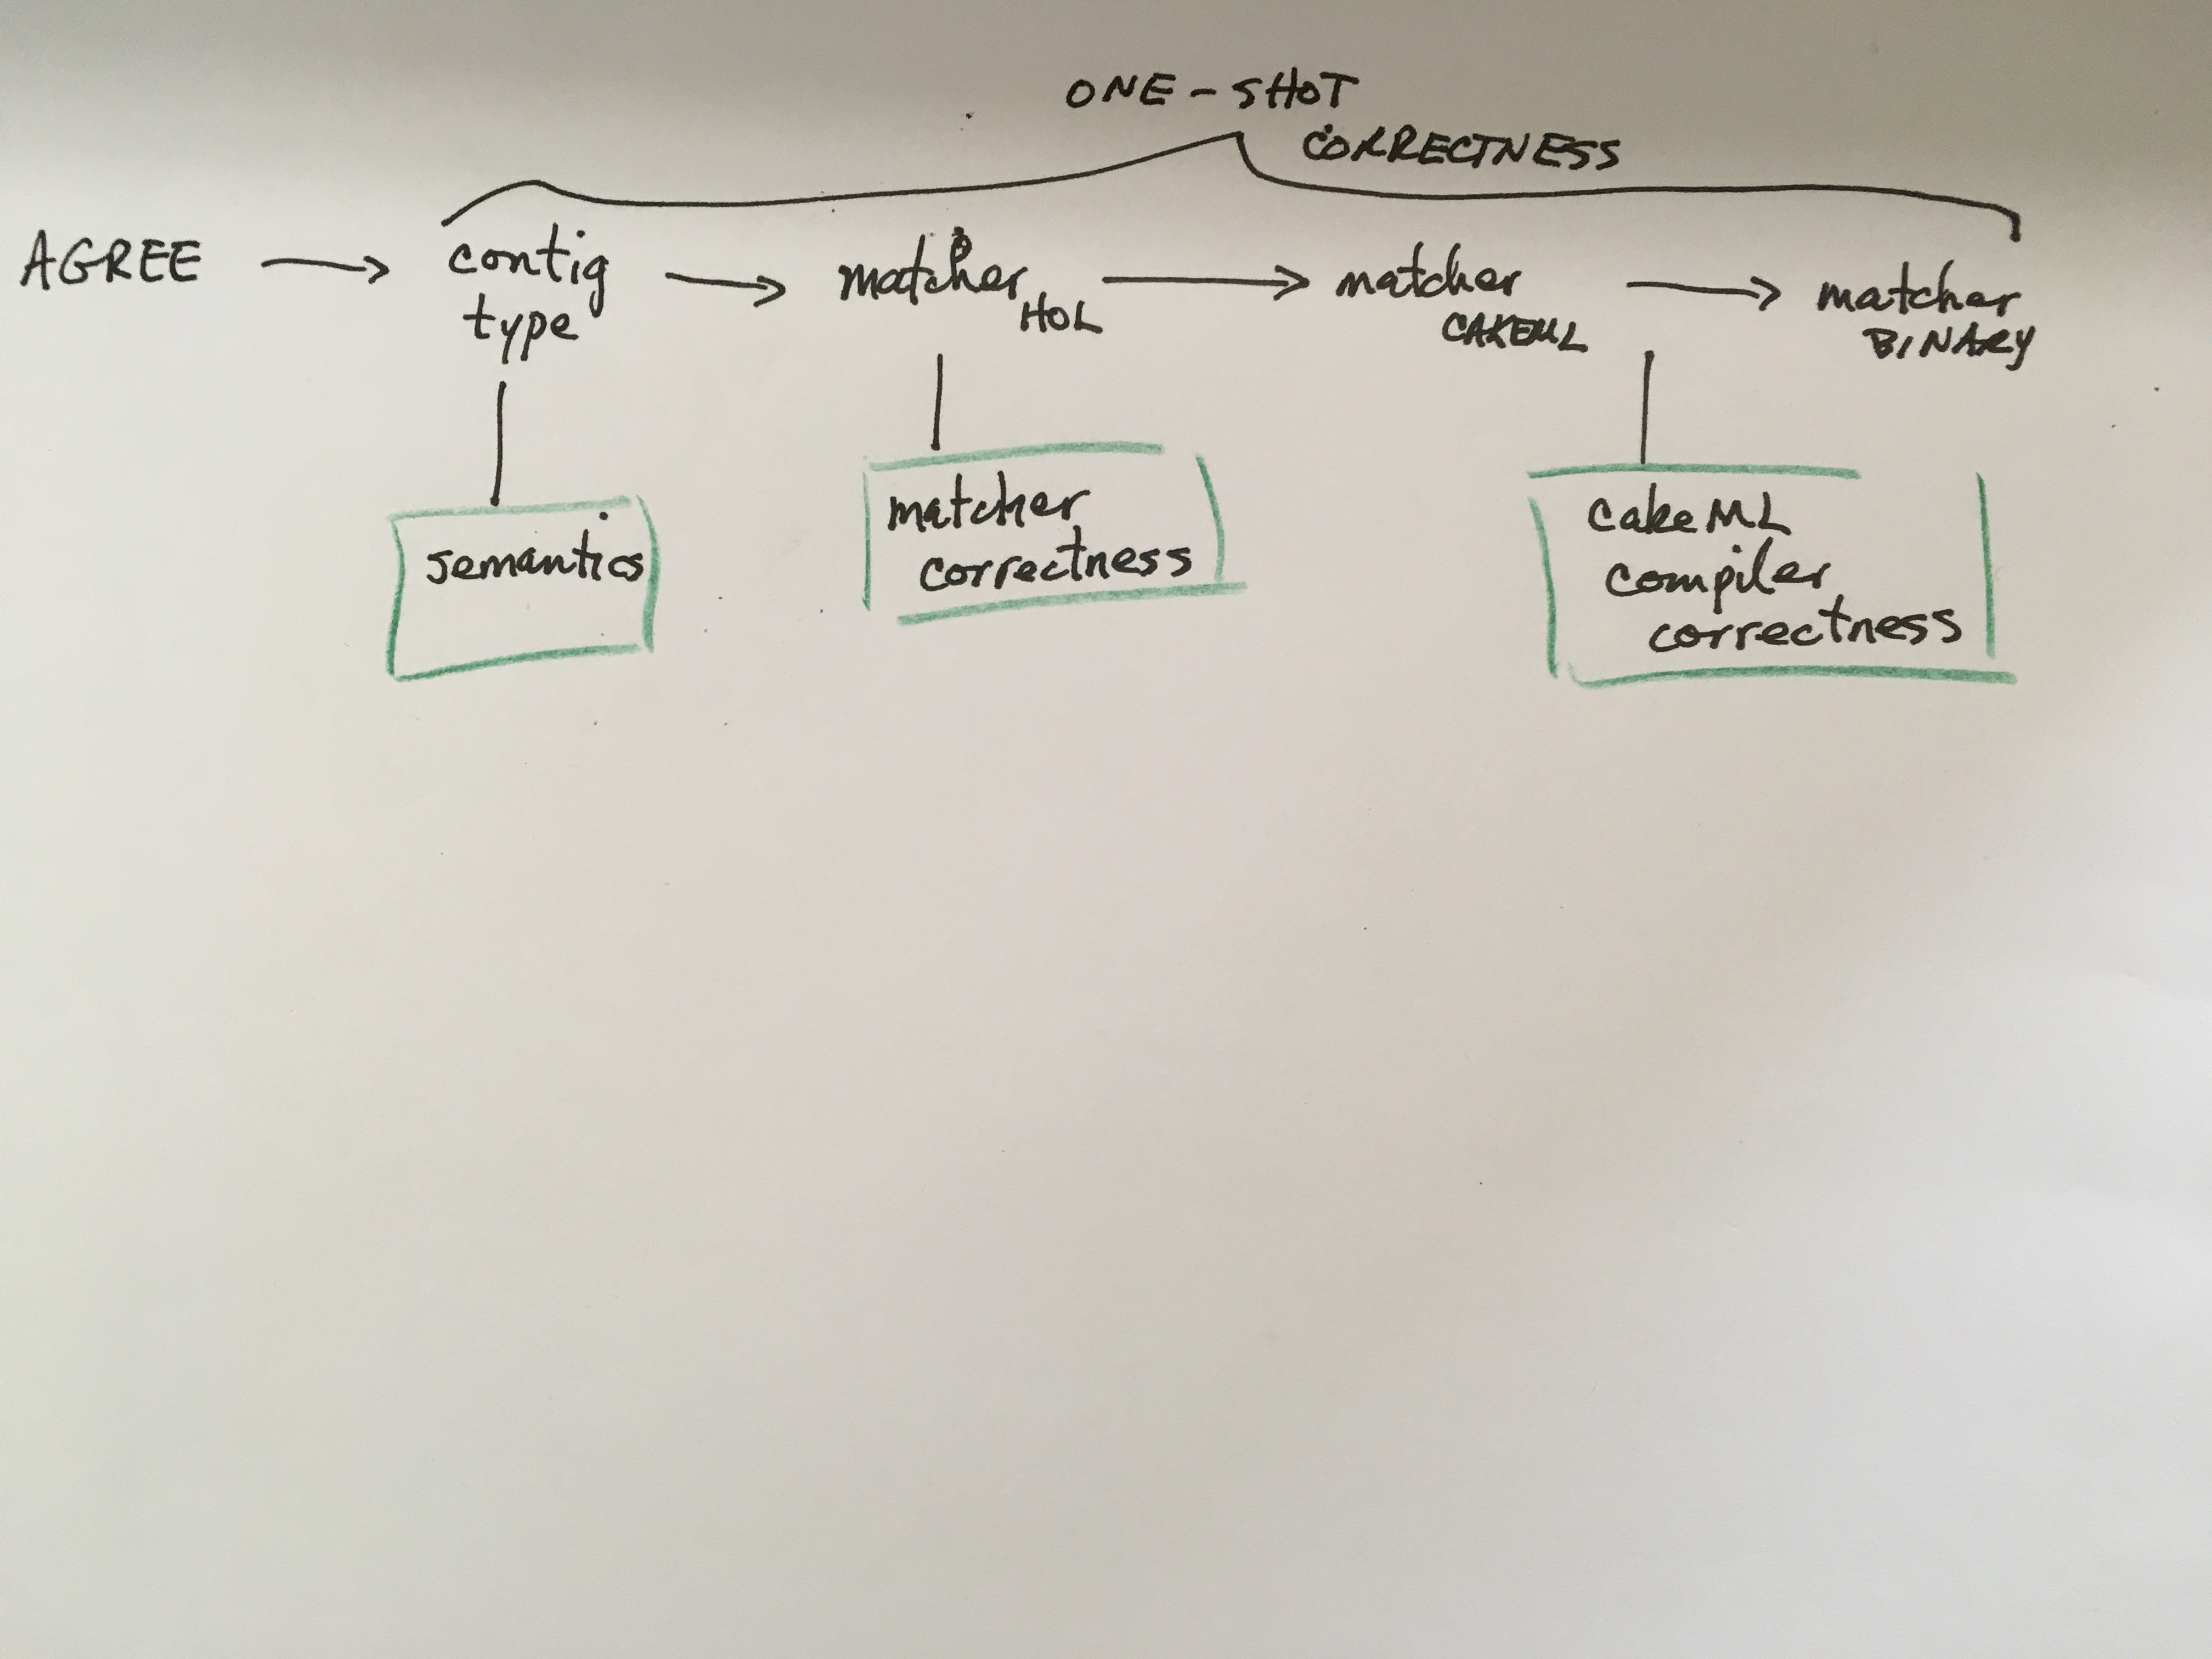
\includegraphics[width=90mm,height=50mm]{one-shot.jpg}

\end{frame}

\begin{frame}\frametitle{Question: value of end-to-end verification}

Q: What is the value of combining verified programs with a verified
   compiler to get a property of the compiled program?

A: It removes places to look for bugs. Instead, the assumptions of
the final joined-up theorem reveal the limitations on applicability.

\end{frame}


\begin{frame}\frametitle{Thread level correctness}

  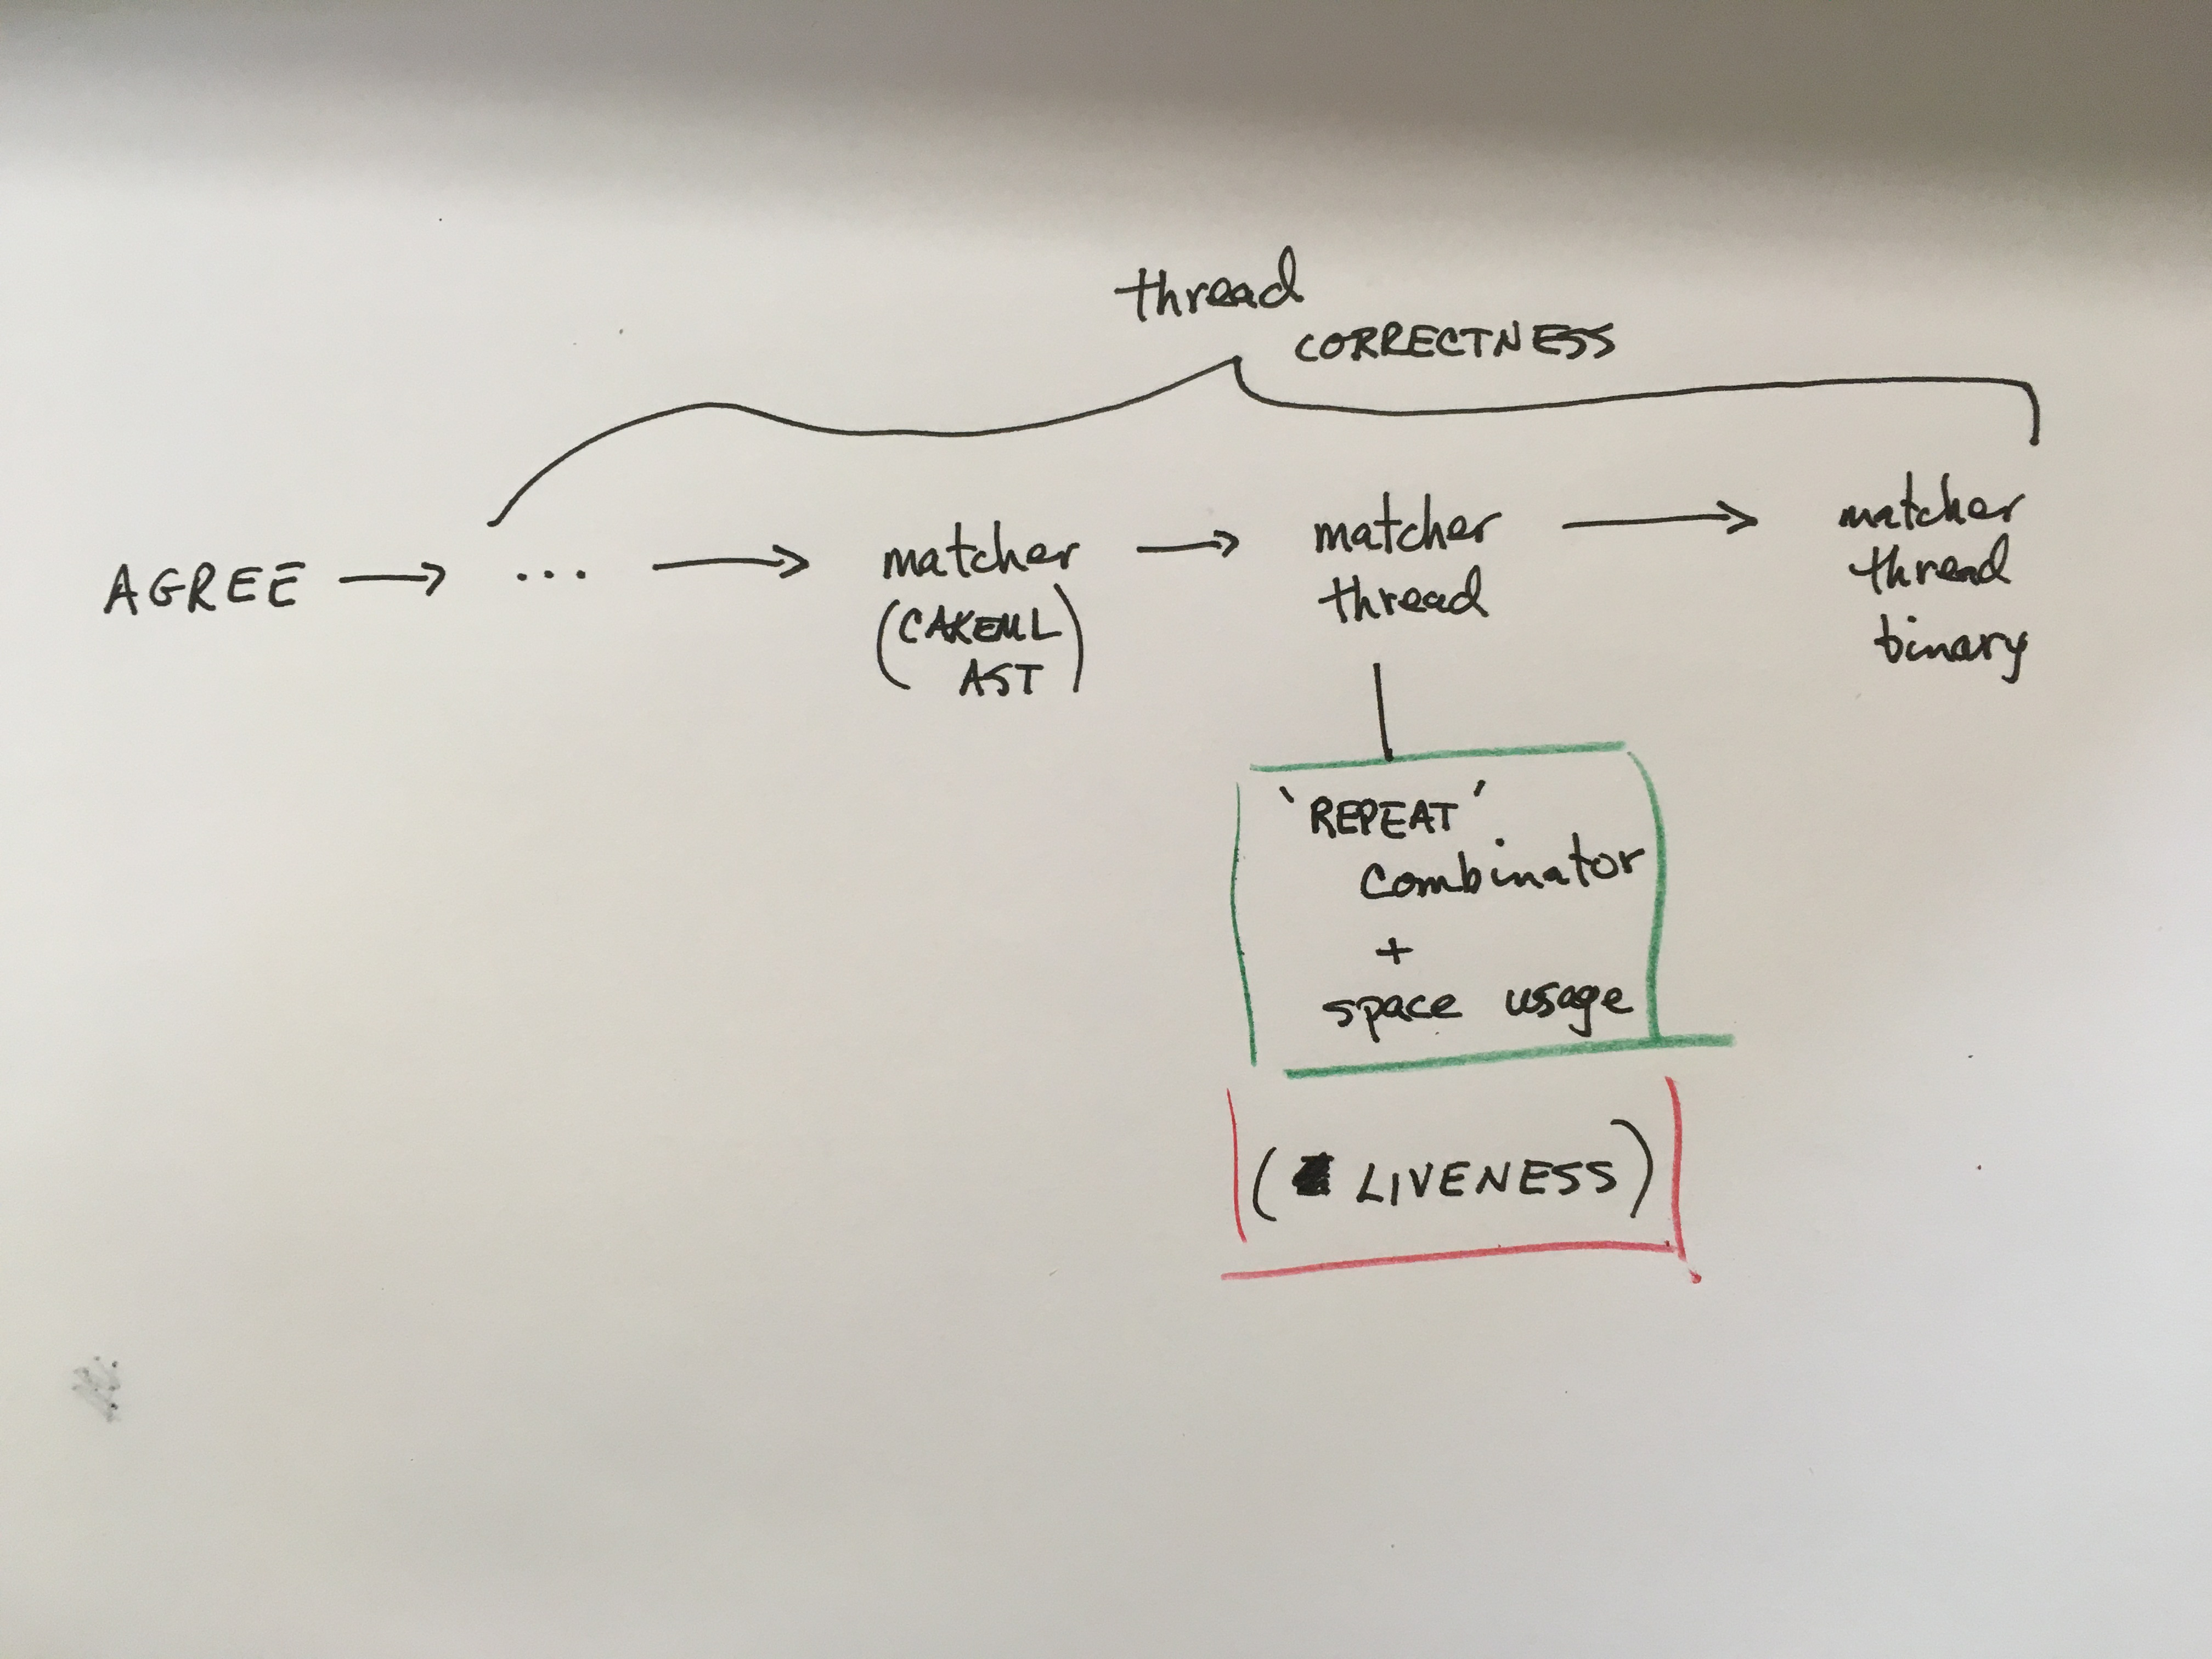
\includegraphics[width=90mm,height=50mm]{thread.jpg}

\end{frame}

\begin{frame}\frametitle{System-level correctness}

Recall \textbf{NEAT}:
  \begin{itemize}
   \item Non-bypassable
   \item Evaluable
   \item Always invoked
   \item Tamper proof
 \end{itemize}

  Desirable properties for our implementation!

We already `have' some of these :

  \begin{itemize}
   \item Non-bypassable
   \item Evaluable (Proofs)
   \item Always invoked (Liveness)
   \item Tamper proof (seL4)
 \end{itemize}

\end{frame}

\begin{frame}\frametitle{System-level correctness}

Note: Non-Bypassability is a system-wide property which depends on the
implementation rigorously obeying the boundaries in the model

Also the vast iceberg of the security properties that seL4 implements
need to be brought into the picture.

Problem: Disparate evidence supporting our security claim.

Solution: Represent the security argument in Resolute

\end{frame}


\begin{frame}\frametitle{Comments and TODO}

\begin{itemize}
\item Start off by giving thanks to the organizers
\item Goes too fast into details; give a more gradual approach to SysArch concept
\item Slide 12 (too many acronyms)
\item Too much text (needs more pictures)
\item Use material from earlier presentations from Isaac and Darren
\item ``Now we implement'' Mark a definite shift from transformations to implementations.
\item Define Tamper-proof
\item Explain ``What is the significance of end-to-end correctness proofs?''
\item Role of HAMR + Adventium stuff
\item Shout-outs to both Kansas places.

\item Be crisper on Non-Bypass vs Always invoked (AInv is not
  liveness; it's liveness plus the fact that it obeys its spec (by
  output being equal to filter function applied to its input)). In
  other words, the filter function can't just output well-formed data:
  the output stream has to be the filtered input stream.

\item Try to express the entire assurance case in a picture: ``it's
  the original system, except safer in the following ways''

\item Map from AADL-->Camkes-->seL4
\item Where we are; what's next

\end{itemize}
\end{frame}

\end{document}
